%!TEX root = Constructive Alignment for Introductory Programming.tex

\chapter{Supporting the Curriculum with Tools and Technologies} % (fold)
\label{cha:supporting}

\graphicspath{{Figures/Supporting/}}

In addressing the need to be agile and willing to change, \pref{itm:agile}, the model from \cref{cha:approach} proposed the separation of teaching and learning activities from resources used to support these activities. This separation aimed to enable greater flexibility in the activities, which were then supported by more generally targeted resources.

\cref{cha:example_impl} outlined the teaching and learning activities for two example implementations of the proposed model from \cref{cha:approach}. The teaching and learning activities discussed in \cref{cha:example_impl} were supported by a number of tools and resources, and these resources are the topic of this chapter.

Resources described in this chapter include tools to support both \emph{how}, and \emph{what}, we taught. \sref{sec:doubtfire} describes an online tool used to support the teaching and learning environment, providing support for \emph{how} the units were taught. \sref{sec:arcana}, \sref{sec:vodcasts} and \sref{sec:swingame} describe three different resources used to support \emph{what} we taught. \sref{sec:arcana} describes a programming text that was used to support the concept-based approach, providing students with details in order to support the concept focused lectures. These details were also provided as a series of video podcasts on language syntax, as outlined in \sref{sec:vodcasts}. Providing general support for what we taught, \sref{sec:swingame} describes a game development framework used to enable students to create more engaging programs.

% section supporting_how_and_what_we_teach (end)

\section{Visualising Progress to Support Formative Feedback} % (fold)
\label{sec:doubtfire}

% \subsection{Background} % (fold)
% \label{sub:doubtfire_background}

Formative feedback, \pref{itm:formative}, plays an important role in shaping the teaching and learning environment for the units implemented using the model presented in \cref{cha:approach}. This change helps support the focus on students active construction of their own knowledge, \pref{itm:construct}, but provides an additional challenge as students no longer have marks to guide their behaviour. To help address this challenge, an online task tracking system, named ``Doubtfire'', was developed. 

Doubtfire allowed each student to track their progress against the weekly assessment tasks using a ``burn down chart'' as shown in \fref{fig:example_chart}, a technique adapted from the Scrum agile software development process \cite{Schwaber:2002}. The charts show the cumulative amount of work remaining week by week, which decreases as work is complete, or burns down over time.

\begin{figure}[thb]
  \centering
  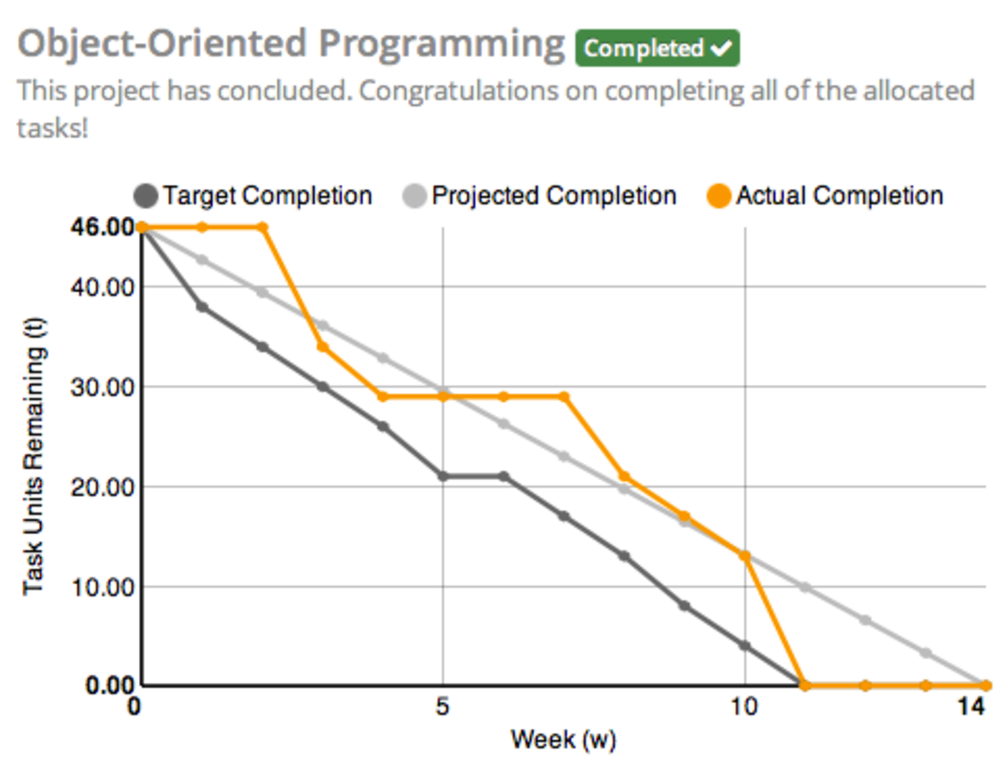
\includegraphics[width=0.9\textwidth]{ExampleChart}
  \caption{An example burn down chart showing progress against weekly tasks.}
  \label{fig:example_chart}
\end{figure}

Agile software development methods \cite{Beck:2001} embrace change \cite{Beck:2000} by allowing for adaptive, periodic adjustment of activities. The basis for this adaptation in Scrum is \emph{empirical} information; a consistent measure of the work remaining (``backlog''), and a measure of the rate work is being completed by the team (``velocity'').

The purpose of a Scrum ``burn down chart'' is to allow stakeholders to consider, in an empirical manner, the velocity of the team with respect to the current backlog. This chart acts as a ``information radiator'' \cite{Cockburn:2002} for the team, providing details on either release or ``Sprint'' iteration schedules. Since quality of work should not be compromised, the requirements (backlog) of work can be adjusted in order to meet the required schedule and cost~\cite{Sutherland:2007}.

In adapting burn down charts as a tool for supporting students engagement with formative assessment tasks, the assessment tasks become the ``backlog''. Students are then able to see the number of tasks remaining, and use their current ``velocity'' to determine if their progress is sufficient to complete the unit on time.

% subsection background (end)

\subsection{Requirements} % (fold)
\label{sub:doubtfire_requirements}

The central requirement for the Doubtfire tool was to provide students with visual feedback on their progress using burn down charts. The burn down charts provide students with a visual representation of the tasks they need to complete over the teaching period, and show the number of tasks, their scheduled due date, and estimated task effort. Students should be able to use the tool to assess their progress throughout the teaching period, and to determine whether they need to increase their rate of progress (velocity) and, if so, commit more time to the unit or take greater advantage of resources available to them. 

It was also seen that the scrum-style marking of tasks as completed could be extended to allow students to indicate if they were working on, or having trouble with, particular tasks. This requirement aimed to increase student engagement with the tool, and improve likelihood that they would make active use of it throughout the teaching period.

To account for task heterogeneity, staff needed to be able to set a specific \emph{weight} for each task. This weight represents the estimated effort students needed to expend to satisfactorily complete the task. Rather than specifying task weight in terms of hours, this was done in a more abstract unit. One popular approach with agile software development projects is to assign tasks ``\emph{t-shirt size}'' weights \cite{Peixoto:2010}. Using this approach tasks have their weight set to a common t-shirt size: \emph{extra small}, \emph{small}, \emph{medium}, \emph{large}, \emph{extra large} etcetera. The t-shirt sizes are then allocated weights, with each increment in size doubling the associated weight: extra small had a weight of one, small a weight of two, medium four, etcetera.

Task weights needed to be incorporated into the burn down chart, with each chart showing the cumulative number of \emph{task-points} remaining. Using task-points in the burn down charts enables the chart to visually show weeks where more, or less, effort is likely to be required.

Progress also needed to be projected to indicate an expected completion date. This projection can be calculated from the average number of task-points the student completes each week.  For example, if six task-points were completed in one week, based on the velocity, a thirty-six task-point project is expected to be completed in six weeks. Each student's projected completion should be recalculated as tasks and weeks progress. 

As an interactive system, Doubtfire had a number of requirements to ensure that it could be best utilised by all targeted users. The following requirements were identified:
\begin{itemize}[noitemsep,nolistsep]
  \item \textbf{Online}: students needed to be able to easily access the tool both in and out of scheduled class times. It was decided to make Doubtfire an online tool, thereby making it accessible from virtually anywhere. It also simplifies the development progress with only web platforms needing to be supported, and avoids the need for students to install client software.
  \item \textbf{Easy to use}: the tool need to be simple enough to use, so the usability of the tools must provide as small a barrier as possible to student adoption.
  \item \textbf{Mobile friendly}: students should be able to quickly check, and update, their progress from a range of devices. Ensuring that Doubtfire can be easily accessed via a mobile device will encourage students to access the tool even when they are away from their computers. 
  \item \textbf{Aesthetically pleasing user interface}: to encourage adoption of the tool among students, a visually appealing user interface is ideal.
\end{itemize}
Simply, our aim was to create a tool that was simple and appealing for students to use and was easily accessible from a range of devices and locations. Students not should feel that interaction with the tool is work.

In addition to students, Doubtfire also addressed needs of teaching staff. Tutors were responsible for managing classes, and therefore needed to be able to respond to student actions in the tool. Convenors had overall responsibility for the unit, and needed to be able to observe the performance of the student cohort and perform simple administrative actions. All teaching staff benefited from the requirements already listed. Most importantly, the mobile nature allowed tutors to easily check and update students' progress during scheduled classes.

\medskip

In terms of the development and deployment of the tool, a number of software qualities are desirable. These include:
\begin{itemize}[noitemsep,nolistsep]
  \item \textbf{Supports the teaching environment}: the tool plays a supportive role, and should therefore fit inside the teaching environment; it should not be necessary to fit the teaching environment around the tool.
  \item \textbf{Quick to develop and extend}: it should be easy to produce features and adapt the tool to ensure it remains relevant to the students.
  \item \textbf{Controllable}: the schema that defines the way tutors and students interact over tasks must be easy to alter to allow for adaptation if assessment criteria change.
\end{itemize}

% It is valuable to add features that track student behaviour in the tool to:
% \begin{itemize}[noitemsep,nolistsep]
%   \item Determine whether the expected use of the software matches the actual.
%   \item Identify possible issues in the unit curriculum, such as inconsistent assignment weighting.
%   \item Identify possible flaws in the rule system governing student and tutor interaction in the software.
%   \item Exploit the information to insights into general teaching issues.
%   \item Optimise the experience based on how students use the software.
% \end{itemize}
% As this information is constantly generated through use of the tool, it is simply a matter of storing what actions have been performed. This provides unambiguous information that can then be analysed through quantitative methods.

% This section has described the requirements we deemed non-negotiable in the production of an effective progress management tool for the users identified. There are a number of minor requirements that were not considered significant enough to describe here. From these requirements were produced a number of features accessible to the convenor, tutor and student user groups, which are discussed in the following section.

% subsection requirements (end)

\subsection{Doubtfire Solution} % (fold)
\label{sub:doubtfire_solution}

\subsubsection{User Roles} % (fold)
\label{sub:user_roles}

The three user groups in Doubtfire were Convenor, Tutor and Student. Each of these groups had access to a different set of features as described in \tref{tab:user_features}. Convenor and Tutor roles were provided to support teaching staff, with the students having a separate role. 

% This is what can do with the tool
\begin{table}[htbp]
  \renewcommand{\arraystretch}{1.6}
  \centering
  \caption{Available features for each user group in Doubtfire}
  \label{tab:user_features}
  \begin{tabular}{c|p{0.9\textwidth}}
    Role & \multicolumn{1}{c}{Features} \\ \hline\hline
    \multirow{5}{*}{\begin{sideways}\parbox{14mm}{Convenor}\end{sideways}}
    & - \textbf{Unit Administration}: including the ability to enrol students and create tasks. \\
    & - \textbf{Monitor Student Progress}: view distribution of students by progress indicators. \\
    & - \textbf{Monitor Task Progress}: view progress distribution for each of the unit's tasks. \\
    & - \textbf{Examine Student Progress}: view the list of tasks and their associated status by student. \\
    & - \textbf{Update Task Status}: mark student work as complete. \\ 
    & \\
    \hline\hline
    \multirow{2}{*}{\begin{sideways}\parbox{10mm}{Tutor}\end{sideways}}
    & - \textbf{Examine Student Progress}: view the list of tasks and their associated status by student. \\
    & - \textbf{Update Task Status}: mark student work as complete. \\ 
    & \\
    \hline\hline
    \multirow{3}{*}{\begin{sideways}\parbox{11mm}{Student}\end{sideways}}
    & - \textbf{Update Task Status}: mark student work as complete. \\ 
    & - \textbf{Monitor Progress}: view progress on task completion using a burn down chart showing Target, Actual and Projected completion. \\
    & \\
  \end{tabular}
\end{table}

Unit convenors are responsible for the overall delivery and management of the unit. To support this role, Doubtfire provided these users with the tools to set up unit tasks and enrol students. A dashboard provided Convenors with an overview of student progress, and enabled quick access to views of student progress by task, and to individual students via their scheduled class. \fref{fig:dashboard} shows an example overview of students progress for a single unit from the Convenor Dashboard. While, \fref{fig:task_chart_view} shows an example chart that visualises the distribution of student status for each task. In addition to these tasks, Convenors also had the ability to perform the same actions as Tutors.

\begin{figure}[thbp]
  \centering
  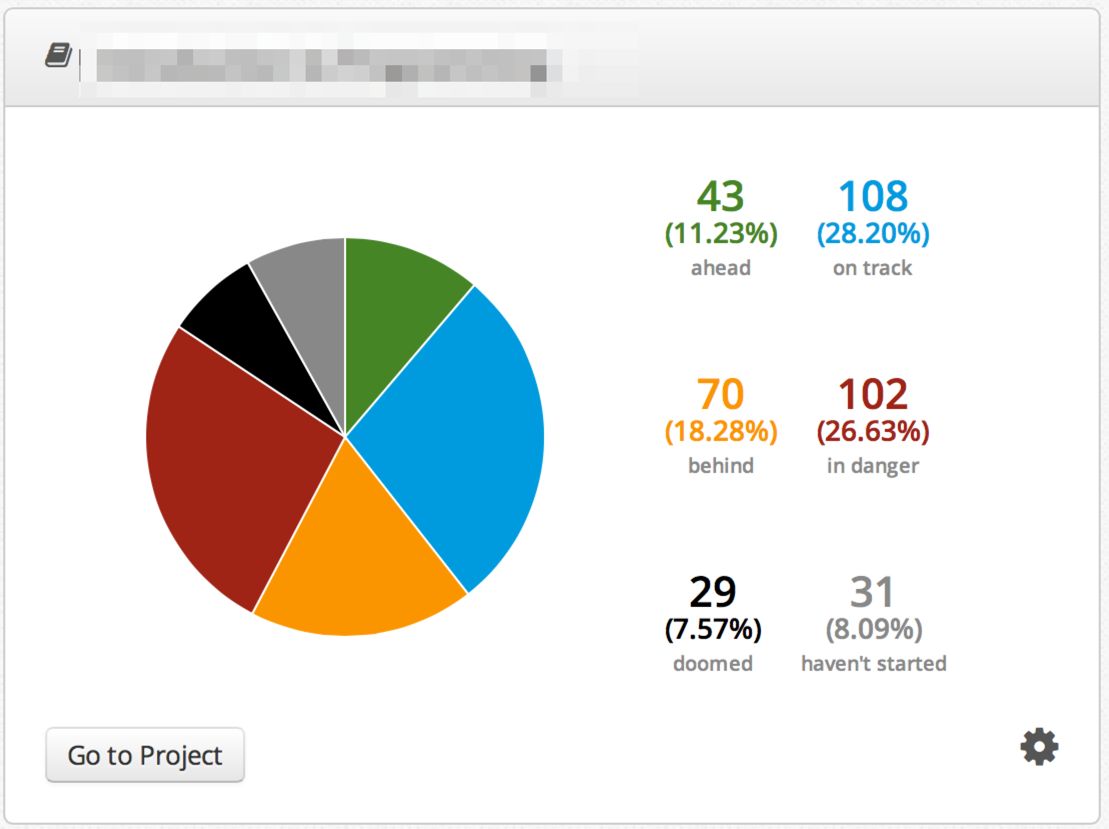
\includegraphics[width=0.8\textwidth]{Dashboard}%
  \caption{Overview of progress by unit from the Convenor Dashboard.}%
  \label{fig:dashboard}%
\end{figure}

\begin{figure}[thbp]
  \centering
  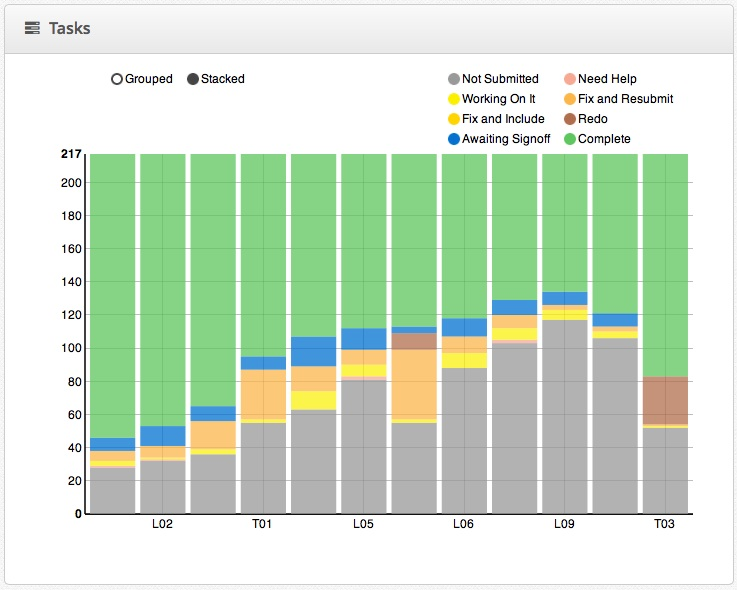
\includegraphics[width=0.8\textwidth]{TaskChart}%
  \caption{Convenor view showing distribution of student status by task}%
  \label{fig:task_chart_view}%
\end{figure}

Tutors are responsible for conducting the tutorial classes, and providing formative feedback for the students in these classes. To support this role, Doubtfire provided tutors with a class list view showing student progress. From the class list, tutors could drill down to view individual students and their burn down charts, and provided a convenient means of updating task status. 

\fref{fig:tutor_view} shows an example of the class list used by Tutors. The class list shows the students in the tutors class, their names and id numbers have been obscured in \fref{fig:tutor_view}, with each task being represented by a coloured rectangle indicating the current status of the task for that student. Tutors are able to update the status of a student's tasks directly from the class list.

\begin{figure*}[thbp]
  \centering
  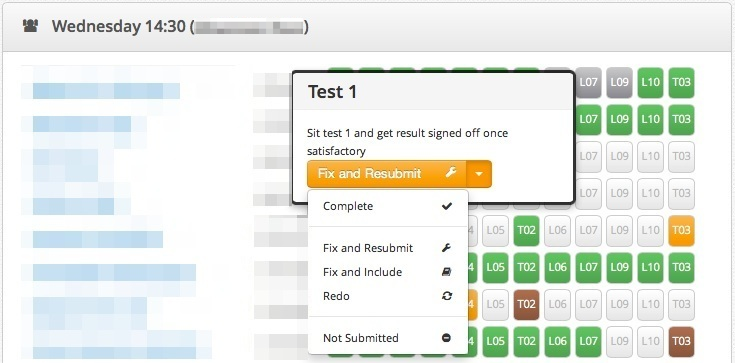
\includegraphics[width=0.8\textwidth]{TutorView}
  \caption{Tutors viewed class groups and could adjust task states}
  \label{fig:tutor_view}
\end{figure*}

\fref{fig:home_page} shows an example of the dashboard provided to students. Each student was provided with a dashboard showing their progress for the units they were enrolled in. Students could view their burn down chart and task statuses by selecting units from their dashboard. When viewing a unit, students could update the status of their tasks as shown in \fref{fig:task_list}.

\begin{figure*}[thbp]
  \centering
  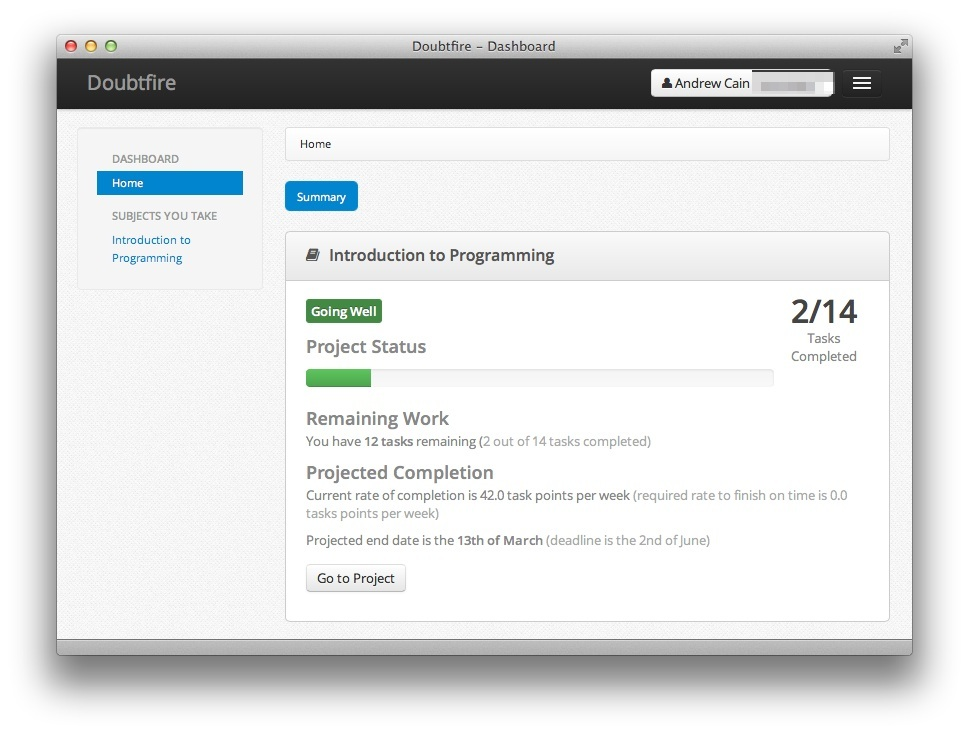
\includegraphics[width=0.8\textwidth]{HomePage}%
  \caption{Student home page in Doubtfire, showing progress on all enrolled projects}%
  \label{fig:home_page}
\end{figure*}

\begin{figure}[thbp]
  \centering
  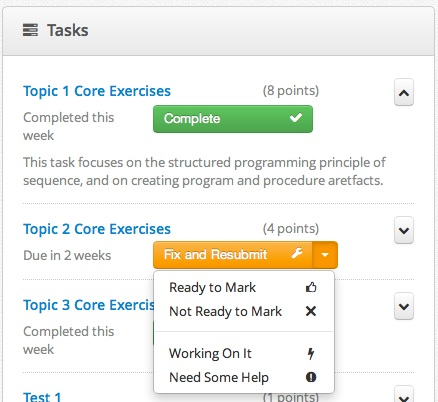
\includegraphics[width=0.6\textwidth]{StudentTasks}
  \caption{The Tasks list enabled students to view and change task status}
  \label{fig:task_list}
\end{figure}

Student progress could be viewed as a burn down chart that consisted of three lines, as shown in \fref{fig:example_chart}. The lines indicated:
\begin{itemize}[noitemsep,nolistsep]
  \item \textbf{Actual Completion}: showed the number of task-points signed off for the student by week.
  \item \textbf{Target Completion}: showed the recommended schedule from the task due dates set by the convenor.
  \item \textbf{Projected Completion}: indicated the current velocity, which was then projected to indicate an expected end date if current velocity was maintained.
\end{itemize}

% subsection user_roles (end)

\subsubsection{Task Processes} % (fold)
\label{sub:task_processes}

Tasks in the Doubtfire system could have one of a number of statuses, with different users being responsible for updating task statuses at various times during unit delivery. The main statuses and the transitions between these is shown in \fref{fig:basic_process_chart} as a UML State Chart. 

\begin{figure}[thbp]
  \centering
  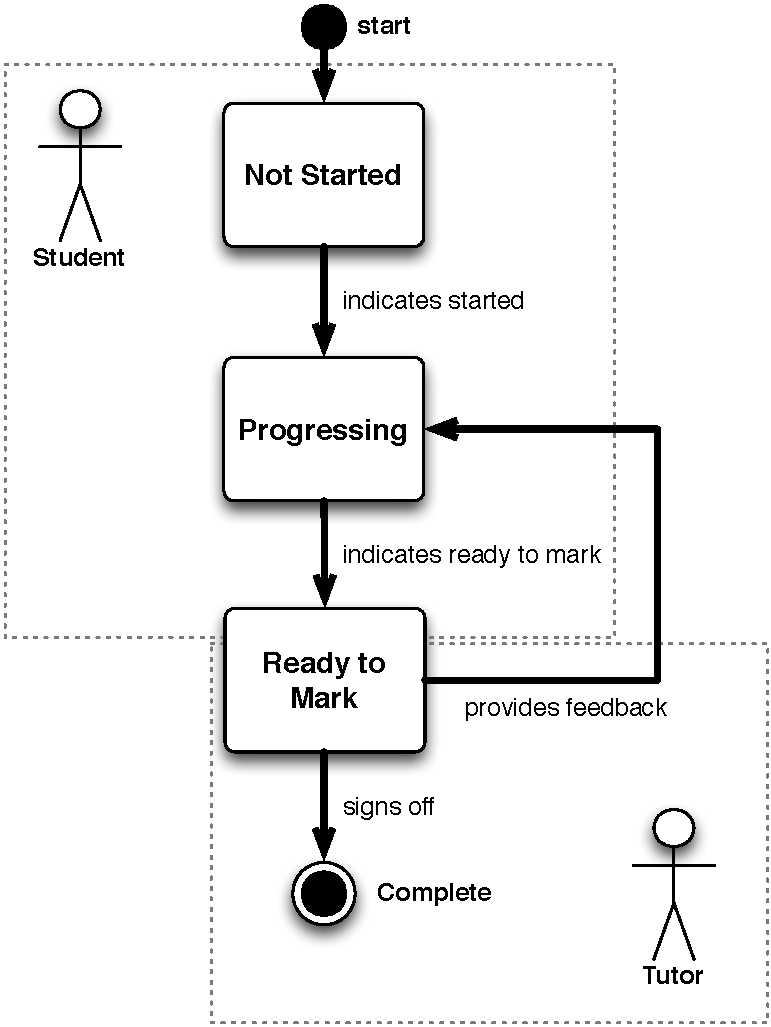
\includegraphics[width=0.7\textwidth]{BasicProcessStateChart}
  \caption{UML state chart showing task states and transitions.}
  \label{fig:basic_process_chart}
\end{figure}

Initially all tasks are set to the \emph{Not Started} status. When students begin work on the task they are encouraged to update its status to \emph{Progressing}, and when it is ready for assessment to the \emph{Ready to Mark} status. Once tutors receive the work, they examine the work and provide the student with formative feedback. After having discussed the task with the student, the tutor updates the status by either returning it to a \emph{Progressing} status if the task needs to be fixed, or signing the task off as \emph{Complete}.

The \emph{Progressing} status was divided into a number of sub-states for the purpose of providing students with finer-grained feedback. 

Students were able to set the status of a task to \emph{Working on It} or \emph{Needs Help} to indicate their current progress on the task to their tutor and to the unit convenor. \emph{Fix} and \emph{Redo} statuses could be used by students to indicate that tasks needed some aspects adjusted (the \emph{Fix} status) or that it should be redone (the \emph{Redo} status). These status, shown in \fref{fig:detailed_states}, were designed to help provide more accurate details of progress for both staff and students. Students indicated how they were progressing with the tasks, and staff could provide feedback on the outcomes students had achieved.

\begin{figure}[thbp]
  \centering
  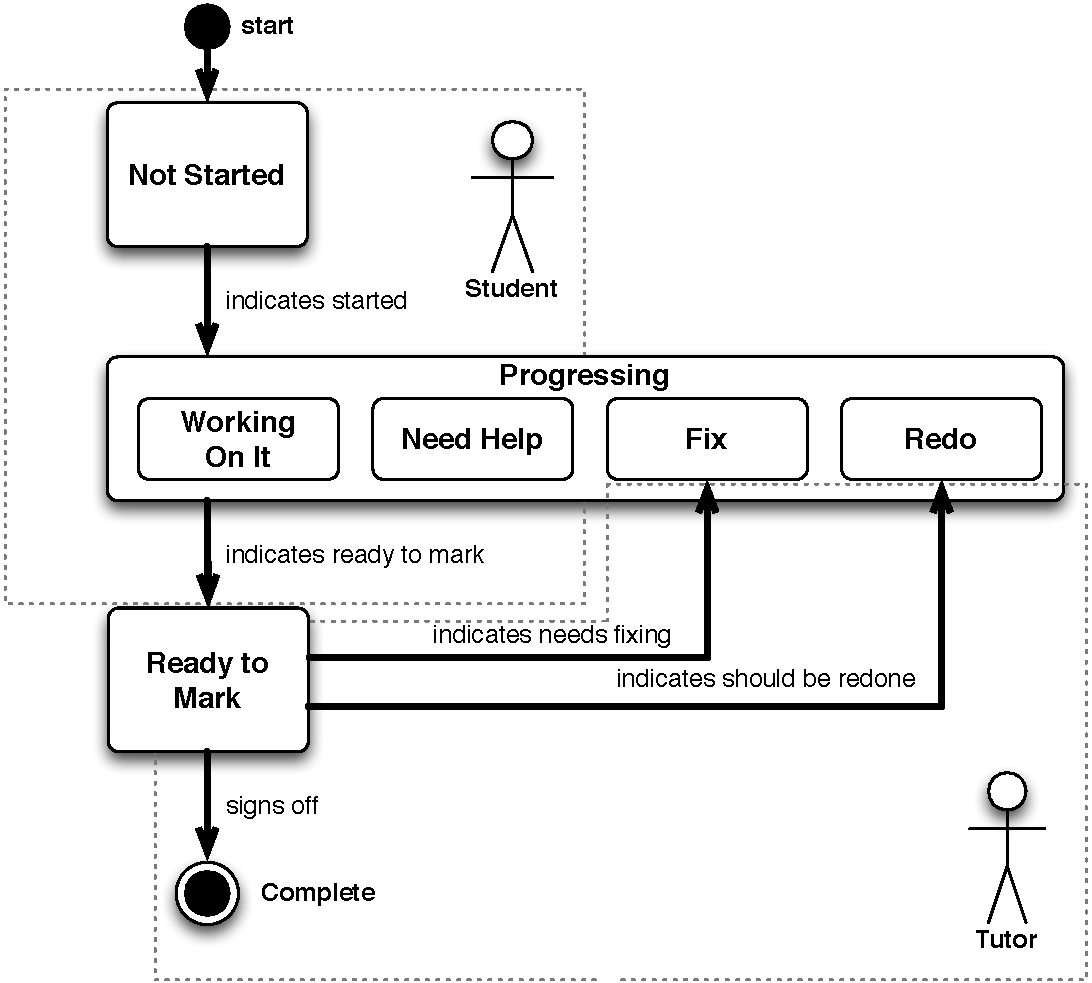
\includegraphics[width=\textwidth]{DetailedStepsInProgress}
  \caption{UML state chart showing the detailed states within the Progressing superstate.}
  \label{fig:detailed_states}
\end{figure}

% subsection doubtfire_solution (end)

\subsection{Use of Doubtfire} % (fold)
\label{sub:use_of_doubtfire}

While \cref{cha:evaluation} provides a more in-depth discussion of the use of Doubtfire, this section will briefly comment on how it was used in the delivery of both the introductory programming and object oriented programming units. In both cases the teaching and learning activities from \cref{cha:example_impl} were used as the tasks to be completed, and teaching staff assigned each a weighting to represent its relative size.

The effectiveness of the tool, for students, depended on their engagement with the unit. The more capable students made active use of Doubtfire, and responded quickly to addressing issues and closing gaps in their knowledge. Students who struggled to complete the weekly tasks generally made poor use of the tool at the start of the teaching period, but engaged actively later in the semester. While some, more disengaged, students avoided use of the system and attempted to establish progress on their own terms. 

For teaching staff, the Doubtfire tool provided useful information on how students were engaging with the formative process. It was easy to see which students were doing well, to identify those who were falling behind, and those who were not engaging with the unit at all. This information was used to prompt students, encouraging those who were doing well and suggesting appropriate resources for those who were falling behind.

\subsection{Summary} % (fold)
\label{sub:doubtfire_summary}

The strong use of formative feedback in the model provides a challenge as students cannot be motivated by marks during the teaching period. This could lead to students allocating insufficient time to complete the unit's tasks, allowing them to fall behind in the unit.

Doubtfire helped to address this concern through the use of burn down charts that visually represented the amount of work students had remaining in the unit. By using this tool staff and students were able to monitor progress throughout the teaching period.

% subsection summary (end)

% section doubtfire_using_burndown_charts_to_support_formative_feedback (end)

\section{Programming Text to Support Concept-Based Approach} % (fold)
\label{sec:arcana}

Concepts were central to \emph{what} we aimed to teach. \pref{itm:concepts} indicates that we should aim to focus on concepts over language syntax. In addressing this principle the programming units from \cref{cha:example_impl} had little, if any, coverage of syntax in the lectures, leaving these details instead to teaching and learning resources. While concepts are important, syntax details are need to enable students to turn these concepts into working code.

One of the central ideas of ``Beyond Bullet Points'' is to fully document the notes attached to a presentation's slides \cite{Atkinson:2007}. In effect, the details are moved from the slide itself to the slides' notes, which can then be printed as an informative handout. In our approach this worked against \pref{itm:agile}, and would have resulted in significant effort being expended on the creation of each week's presentation, thereby adding resistance to change if they were found to be ineffective.Instead of documenting these notes in the presentations themselves, they were written up in a separate resource which became the ``\emph{Programming Arcana}'' \cite{Cain:2013arcana}.

Documenting the language details in a separate text also helped to address another issue raised as a result of choosing Pascal as one of the programming languages. Pascal is not currently a popular language with text book writers, and while the Free Pascal Language Reference Guide \cite{FPC:2013lang} provides details of the language it is not designed for beginners.


\subsection{Chapter Sequence} % (fold)
\label{ssub:chapter_sequence}

Chapters in the Programming Arcana were designed to align with the main concept topics from the introductory programming unit. This meant that the text needed to embody the concepts-first approach, \pref{itm:concepts} discussed in \cref{cha:guiding_principles}. To best support this, each chapter needed to focus on providing a coherent set of concepts that built upon concepts presented earlier in the text. The following list illustrates how the programming concepts are presented in the Programming Arcana. This is followed by a discussion of how well the text was able to embody the concept first approach.

\begin{enumerate}[noitemsep,nolistsep]
  \item \textbf{Building Programs}: introduced students to the tools they required, and showed them a basic program they could compile to check the tools were working. The concepts in this chapter included: 
  \begin{itemize}[noitemsep,nolistsep]
    \item \textbf{Programs} were introduced as a sequence of instructions that get the computer to perform actions.
    \item \textbf{Machine and Assembly code} provided some context as to why compilers are necessary. Machine code was presented as the computers natural language, and Assembly as a first step toward making this code more human-friendly.
    \item \textbf{Source code and compilers} introduced the ideas of third generation languages, and the need for a compiler to convert this code to machine code.
    \item The \textbf{Terminal} was introduced as a means of running programs, and the steps for using the compiler were presented. This section also introduced the \textbf{BASH} shell, along with commands to navigate through the file system. 
    \item The final concept outlined the code for a \textbf{Hello World} program in C and Pascal, together with the steps needed to compile and run this program. 
  \end{itemize}
  \item \textbf{Program Creation}: described how code could be written to create a \emph{Program}.
  \begin{itemize}[noitemsep,nolistsep]
    \item This introduced the idea that a \textbf{Program} could be created in code, and that it had a name and a list of instructions for the computer to perform.
    \item \textbf{Procedures} were introduced as a named group of instructions that performed a task. These instructions could be run using a \textbf{Procedure Call}.
    \item The idea that procedures could be distributed in a \textbf{Library} was introduced.
    \item Programming language terminology was also introduced, include \textbf{Statements} as the technical term for commands, \textbf{Expressions} for calculated values, \textbf{Types} to describe different kinds of data, and \textbf{Identifiers} as the names for artefacts such as the programs created and the procedures called. 
    \item \textbf{Comments} were also discussed as a means of documenting code.
  \end{itemize}
  \item \textbf{Procedure Declaration}: introduced the idea that you can create your own procedures to encapsulate the steps of a task. 
  \begin{itemize}[noitemsep,nolistsep]
     \item \textbf{Procedure declaration} described how procedures could be created as a sequence of instructions that are run when the procedure is called.
     \item The concept of a \textbf{Program} was extended to indicate that a program's code could include procedure declarations.
   \end{itemize} 
  \item \textbf{Storing and Using Data}: made programs more dynamic with variables and constants to store data, and functions to calculate values.
  \begin{itemize}[noitemsep,nolistsep]
    \item \textbf{Variables} were introduced as a means of storing data that changed within the code, while \textbf{Constants} were introduced as a means of storing data that does not change. 
    \item The \textbf{assignment statement} was introduced as the means of storing a value in the variable, and the concept of an \textbf{expression} was updated to indicate it could read the value from the variable.
    \item Programming terminology related to the location of a variable was introduced, with \textbf{local variables} being declared within a procedure, \textbf{global variables} within the program, and \textbf{parameters} as a means of enabling data to be passed to a procedure.
    \item The different parameter passing options were presented, with \textbf{pass-by-value} indicating that the value of the expression in the procedure call was passed, while with \textbf{pass-by-reference} the parameter needs to be passed a \emph{variable} to which it will refer.
    \item Creating \textbf{Functions} to calculate values was also introduced, along with updating expressions to indicate the use of \textbf{function calls}.
    \item To realise these concepts, the previous \textbf{statement}, \textbf{program} and \textbf{procedure declaration} concepts were updated.
  \end{itemize}
  \item \textbf{Control Flow}: introduced the structured programming principles, along with the control flow mechanisms of selection and repetition.
  \begin{itemize}[noitemsep,nolistsep]
    \item \textbf{Boolean data} was discussed as a means of directing the control flow statements. This included the use of \textbf{comparisons} to calculate boolean values, as well as the \textbf{logical operators} (\emph{and}, \emph{or}, and \emph{not}).
    \item Selection was described in terms of \textbf{branching}, this included the ideas of \textbf{if statements} and \textbf{case statements}.
    \item \textbf{Looping} introduced \textbf{pre-test loops} that repeated code zero or more times, and \textbf{post-test loops} that repeated code one or more times. 
    \item Other control flow statements were covered in the section on \textbf{jumping}. This included \textbf{break} to jump out of a loop, \textbf{continue} to jump to the end of a loop, \textbf{exit/return} to jump out of a function or procedure, and \textbf{goto}.
    \item Finally, the idea of grouping statements in a \textbf{compound statement} was presented, and explained in terms of providing a sequence of statements within the control flow statements.
  \end{itemize}
  \item \textbf{Managing Multiple Values}: presented the use of arrays.
  \begin{itemize}[noitemsep,nolistsep]
    \item \textbf{Arrays} were presented as a means of managing a number of values in a single variable. \textbf{String} was discussed as an example of an array students had already been working with.
    \item The importance of \textbf{pass-by-reference} was reintroduced.
    \item \textbf{For loops} were introduced as a convenient means of looping over the elements of an array. 
    \item The \textbf{Assignment statement} and \textbf{Expression} concepts were updated to indicate how arrays could be used.
  \end{itemize}
  \item \textbf{Custom Data Types}: described how developers can create types to help them organise the data in their programs, much as functions and procedures helped to organise functionality.
  \begin{itemize}[noitemsep,nolistsep]
    \item \textbf{Types} were described again, in more detail to provide context. 
    \item \textbf{Type declaration} was discussed along with \textbf{records/structs}, \textbf{enumerated types} and \textbf{unions}. This required an update to the concept of what a \textbf{Program} can contain.
    \item The \textbf{Assignment statement} and \textbf{Expression} concepts were updated to indicate how the various custom types could be used.
  \end{itemize}
  \item \textbf{Dynamic Memory Allocation}: extended programs beyond the confines of the stack, allowing the allocation of data on the heap.
  \begin{itemize}[noitemsep,nolistsep]
    \item The \textbf{Stack} and \textbf{Heap} were discussed. This highlighted the need for values on the stack to have a known size, requiring another ``space'' for allocating data when its size is not known at compile time.
    \item \textbf{Pointers} were introduced as a means of referring to space allocated on the Heap.
    \item The need for specific actions to \textbf{allocate memory}, and to \textbf{free} that allocation were also presented.
    \item Common \textbf{issues with pointers} were also discussed, indicating why they are likely to occur and how to address these issues. This included \textbf{access violations}, \textbf{memory leaks} and \textbf{accessing released memory}. 
  \end{itemize}
  \item \textbf{Input and Output}: described how to save and load data from file.
  \begin{itemize}[noitemsep,nolistsep]
    \item The concept of \textbf{persisting data} discussed the idea of a process and its memory being freed after the program terminates. This lead to details on saving data from the program's memory onto persistent storage.
    \item \textbf{Files} and text and binary \textbf{file formats} were discussed. 
    \item \textbf{Interacting with Files} described the typical input and output operations you are likely to perform on a file.
    \item \textbf{Other output devices} related the concepts presented to terminal input/output and the idea that the same concepts applied to sending data across a network connection.
  \end{itemize}
\end{enumerate}

In proposing \pref{itm:concepts}, with its focus on programming concepts, \cref{cha:guiding_principles} outlined the requirement that we needed to ``Introduce programming concepts incrementally''. The Programming Arcana provides an example of how the details of the programming language can be presented in such a way as to ensure most topics are presented incrementally, with each topic building upon the previously presented topics. 

There were two cases where concepts could not be suitably explained within the overall context presented in a chapter. Other than these two cases, all other chapters were able to explain all concepts in terms of the presented, or previously presented, concepts.
\begin{itemize}[noitemsep,nolistsep]
  \item In Chapter 1, of the Programming Arcana, a program was given to enable students to compile something before they understood what it represented. However, the main focus of the chapter was the tools being presented and not the program's code. 
  \item Chapters 2 and 3 of the Programming Arcana passed values to procedures before topics related to how data can be stored in a program. The idea that data can be passed to a procedure was covered, but not how that data was received.
\end{itemize}

In general, mapping the concepts to syntax was simpler for the Pascal programming language. The main challenges with the C language\footnote{The C code was compiled with a C++ compiler to add support for function and procedure overloading, and pass-by-reference.} were the standard input and output functions, \texttt{printf} and \texttt{scanf} and associated details such as format strings and pointers, and the need to understand arrays before working with strings. This meant that early topics were reduced to using string literals and limiting variables to working with numeric values. In this way the one example could be mapped to both C and Pascal. 

The use of Pascal in the first part of the unit meant that teaching and learning activities could take advantage of Pascal's more convenient support for strings and terminal input and output. For example, consider a program that asked the user to enter their name and then echoes back a welcome message. In C this requires an understanding of variables, format string syntax, arrays, pointers, and how arrays are automatically passed by references where other types are not. In Pascal the same program only requires an understanding of variables and pass-by-reference.

% \begin{itemize}[noitemsep,nolistsep]
%   \item Introduce programming concepts incrementally;
%   \item Provide students with time to put concepts into practice;
%   \item See syntax as a means to an end, not an end in itself;
%   \item Avoid using language features before concepts that can explain their use; and
%   \item Map concepts to code using programming language grammars.
% \end{itemize} 


% subsubsection chapter_sequence (end)

\subsection{Chapter Layout} % (fold)
\label{ssub:chapter_layout}

Each chapter of the Programming Arcana had a similar sequence to its sections. This aimed to promote a consistent approach to studying each of the topics. In keeping with \pref{itm:concepts}, the concepts were presented as the focus of each chapter. % The was followed with examples of how to apply the concepts, and then the language syntax for C and Pascal. Following this a section was dedicated to tracing the execution of the concepts in a conceptual machine, akin to the notional machine discussed by \citet{DuBoulay:1986}. Each chapter then concluded with examples and exercises.

\begin{enumerate}[noitemsep,nolistsep]
  \item \textbf{Concepts}: each chapter started with a list of related concepts.
  \item \textbf{Applying the Concepts}: following the concepts was an example of applying those concepts in an abstract sense, using pseudocode and flowcharts to illustrate how the concepts could be applied.
  \item \textbf{Syntax in C and Pascal}: details of how to code the concepts were first presented in C, with the following section detailing the syntax for Pascal.
  \item \textbf{Understanding the Concepts}: traced the execution of the pseudocode on a conceptual machine, with the aim of showing students how the concepts are realised at run time. 
  \item \textbf{Examples}: listed a number of examples, each presented in pseudocode then in C and Pascal code.
  \item \textbf{Exercises}: a sequence of exercises students could use to develop their understanding of the topic.
\end{enumerate}

Details of the sections related to presenting the concepts follow. This outlines how the Programming Arcana implemented the concept-based approach, and reinforce the focus on concepts over syntax throughout the material presented. 

\clearpage
\subsubsection{Concepts} % (fold)
\label{par:concepts}

Each chapter started with a section that provided details of the concepts being presented. This section started with a brief overview that described how all of the concepts are related. This was followed by subsections that covered the details of each concept, with a textual description, visual concept map, and a series of notes with important details related to the topic. At the end of the concept section an overall concept map was included that visually showed the relationship between the concepts covered. 

\fref{fig:arcana_concepts} shows an example of the concept of branching from chapter 5 of the Programming Arcana. The diagrams were deliberately drawn using irregular shapes to indicate these were a conceptualisation, rather than an exact representation of the associated concepts.

One of the design goals was to fit each concept on a single page. This goal aimed to help support students active construction of their knowledge, \pref{itm:construct}. Aiming to keep each topic to a single page ensured that we focused on the most important details, and where topics expanded over multiple pages the details were examined to ensure we had not included any unnecessary details.

\begin{figure}[hb]
  \centering
  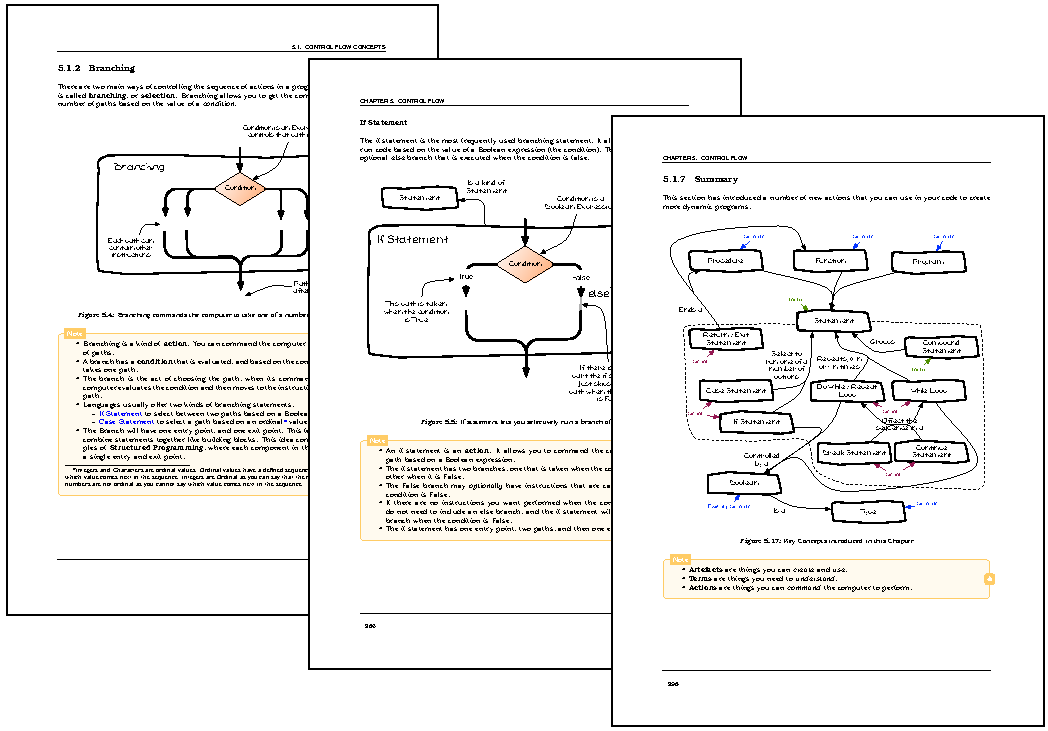
\includegraphics[width=0.7\textwidth]{ArcanaConcepts}
  \caption{Example concept pages from the Programming Arcana.}
  \label{fig:arcana_concepts}
\end{figure}

% paragraph concepts (end)

\subsubsection{Applying the Concepts} % (fold)
\label{par:applying_the_concepts_}

After the concepts were presented, the next section outlined how these concepts could work together to create an example program. This section always started with a specification of a program that was to be created. This was then followed by a discussion of how a the program could be designed using the concepts covered to that point in the text. The description of the design included pseudocode, flow charts, sequence diagrams and structure charts, and the section concluded with a complete design for specified program. \fref{fig:arcana_applying} shows an example of some pages related to applying control flow concepts.

Explanatory text accompanied the design, and highlighted how the concepts covered contributed to the end result. This discussion also presented a way of approaching problems using the concepts to introduce students to the idea of designing their own programs.

\begin{figure}[hb]
  \centering
  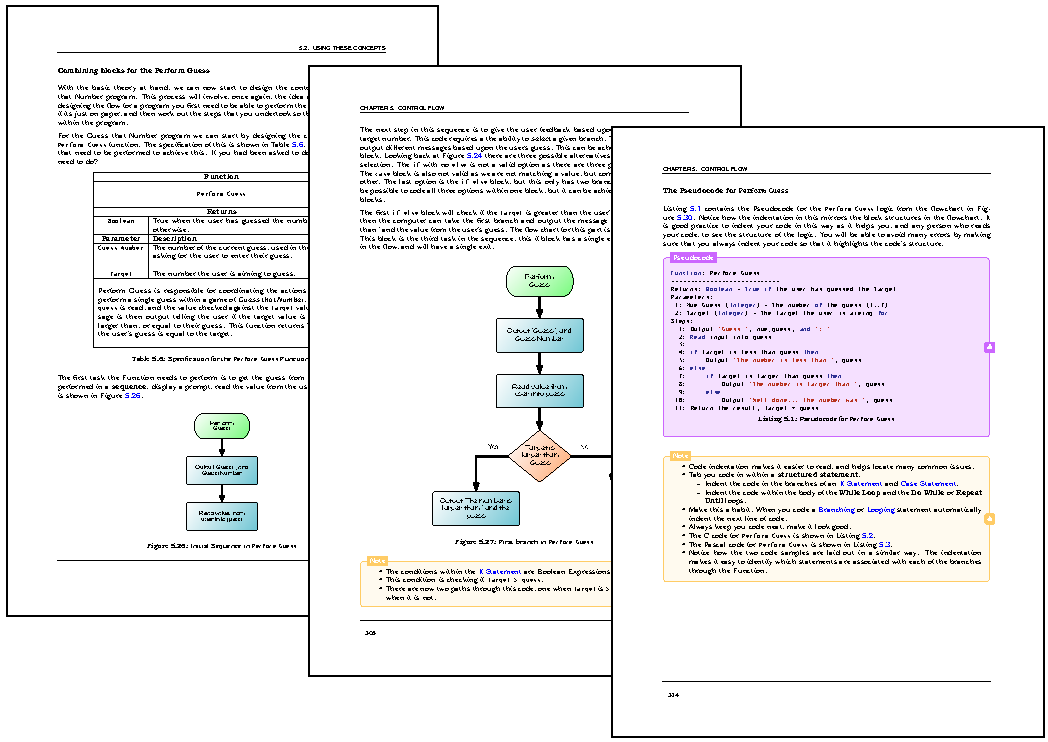
\includegraphics[width=0.7\textwidth]{ArcanaApplying}
  \caption{Example pages related to applying the concepts from the Programming Arcana.}
  \label{fig:arcana_applying}
\end{figure}

% paragraph applying_the_concepts_ (end)

\subsubsection{Syntax} % (fold)
\label{par:syntax}

Having covered the concepts, and how they can be used to create a conceptual program, the next two sections dealt with realising these concepts in C and Pascal code. The syntax sections of the Programming Arcana started with an implementation of the program designed in the section on applying the concepts, which was followed by the grammar to implement the various concepts discussed. An example of pages from this section is shown in \fref{fig:arcana_syntax}.

As with the concepts, the aim was to explain each aspect of the syntax in a single page. This page started with a textual description of the syntax, which was followed by a graphical representation of the grammar and then one or two examples of its implementation in code. The grammar and examples presented focused on best representing the concepts, in many cases only presenting a suitable subset of what was possible with the programming language. 

\begin{figure}[h]
  \centering
  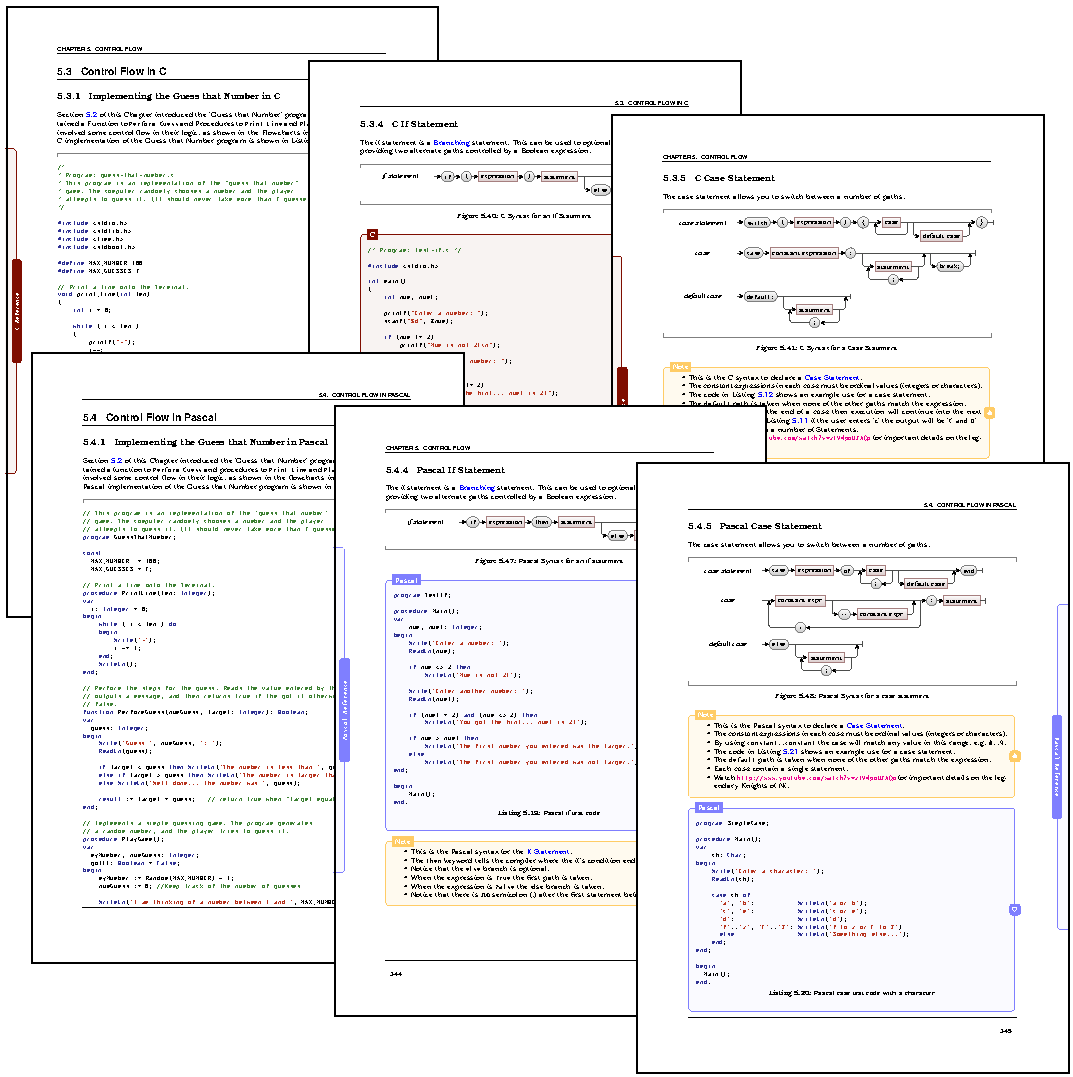
\includegraphics[width=0.7\textwidth]{ArcanaSyntax}
  \caption{Example pages from the Programming Arcana showing C and Pascal syntax and examples.}
  \label{fig:arcana_syntax}
\end{figure}

% paragraph syntax (end)

\subsubsection{Understanding the Concepts:} % (fold)
\label{par:understanding_the_concepts_}

% paragraph understanding_the_concepts_ (end)

Programming has been likened to understanding how to control a notional machine \cite{DuBoulay:1986}. The notional machine represents an ideal computer in which the programming constructs being taught are realised. To help students realise the goal of controlling this machine, the next section of each chapter in the Programming Arcana provided a series of illustrations that tried to communicate the state and behaviour of the notional machine being presented. 

\fref{fig:arcana_understanding} shows some examples from the chapter on control flow. The illustration of the notional machine focuses on memory, and the instruction the computer is executing. Each instruction in the code is executed and explained on a single page.

\begin{figure}[h]
  \centering
  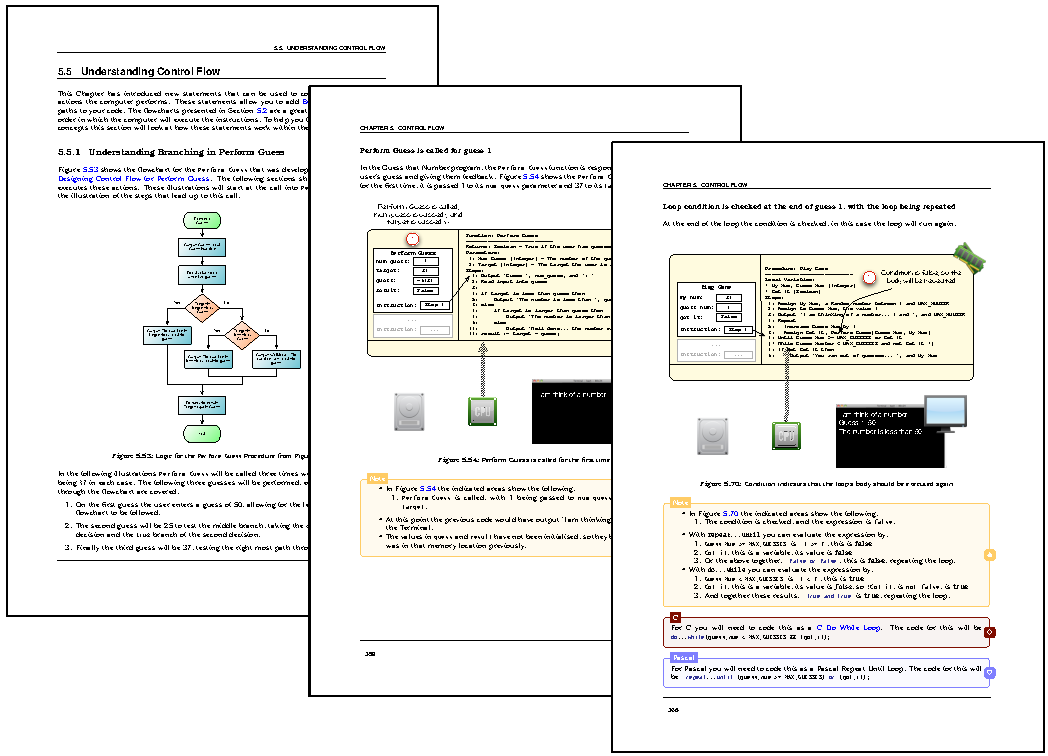
\includegraphics[width=0.8\textwidth]{ArcanaUnderstand}
  \caption{Examples of pages on how the concepts worked at a conceptual level in the machine from the Programming Arcana.}
  \label{fig:arcana_understanding}
\end{figure}

\clearpage

% \begin{figure}[p]
%   \centering
%   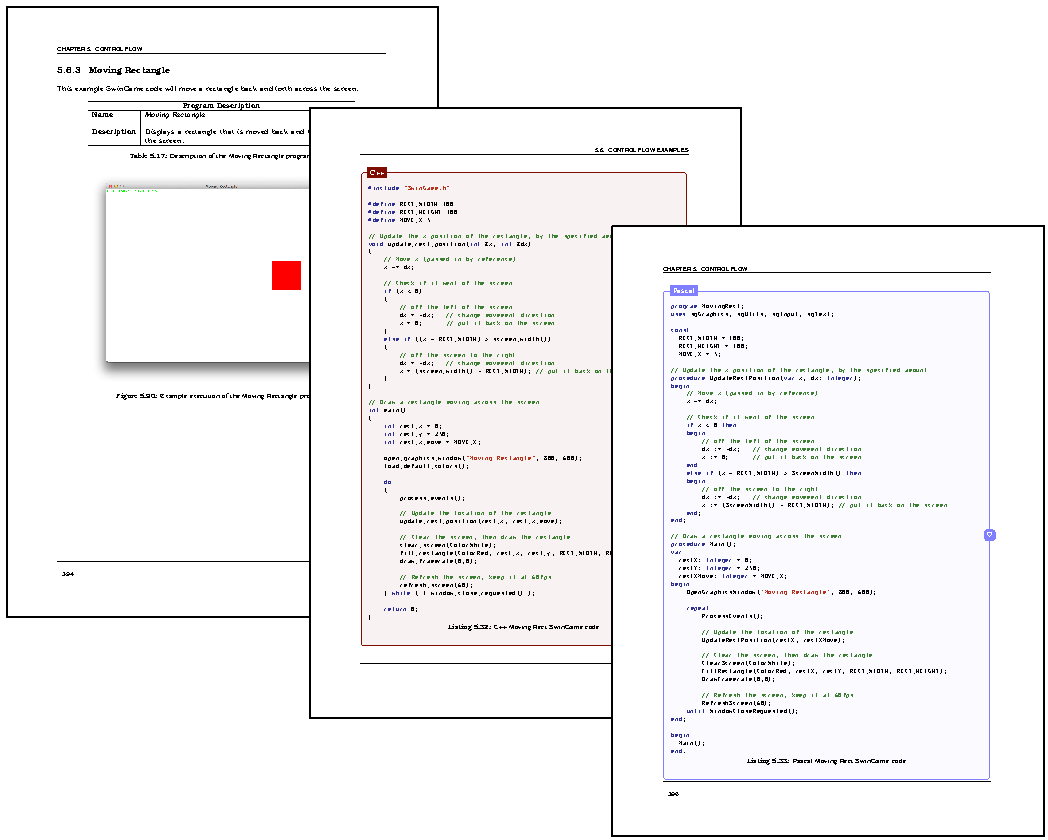
\includegraphics[width=0.8\textwidth]{ArcanaExamples}
%   \caption{Example code from the Programming Arcana.}
%   \label{fig:arcana_examples}
% \end{figure}


% subsubsection chapter_layout (end)


\subsection{Generating Railroad Diagrams} % (fold)
\label{ssub:railroad_diagrams}

Another aim in constructing the Programming Arcana was to provide students with descriptions of the programming language grammar. This could be achieved using a textual representation of the programming language grammar with the Backus Naur Form (BNF) \cite{Backus:1959} or the Extended Backus Naur Form (EBNF) \cite{Wirth:1977}. Instead, it was decided to use the ``Railroad diagrams'' described by \citet{Braz:1990}. These provide a more visual means of presenting the grammar, which was intended to be benefit people reading these diagrams for the purpose of writing programs.

To help automate the creation of the ninety syntax diagrams present in the programming arcana, a language translator was developed to convert grammars expressed textually into a graphical railroad diagram that could be included in the text and lecture slides. 

Originally, grammars expressed in BNF used recursion to implement the repetition of elements in the language. In proposing EBNF, \cite{Wirth:1977} included an iteration construct that reduced the heavy use of recursion for expressing simple repetition of elements in the language. To simplify the generation of railroad diagrams, EBNF was extended further to cater for repeated patterns that included a separator. In BNF and EBNF this can be achieved using recursion, whereas in the railroad diagram the separator should be placed on the returning arrow that implemented the loop. The syntax diagram in \fref{syn:paramlist} illustrates these two approaches. 

\syntax{syn:paramlist}{Examples of the declaration of a parameter list with recursion and without.}{paramlist}

To cater for the more flexible representation in the railroad diagrams, an extended version of EBNF was used. This extension added the ability to indicate a separator for repetitions, and to indicate if the repetition occurred at least once. The grammar for this extended version of EBNF is shown in its own form in \fref{lst:eebnf}, and as a railroad diagram in \fref{syn:eebnf}.

\ebnfsection{lst:eebnf}{Extended EBNF grammar in Extended EBNF}{\ebnfcode{syntax/eebnf.ebnf}}

\syntax{syn:eebnf}{Syntax for grammar used in language diagram generation.}{eebnf}

The \texttt{+ | *} after the repetition indicates either that the grammar had to be repeated one or more times (\texttt{+}) or zero or more times (\texttt{*}). The optional group following this indicated the presence of a separator, between each repetition of the grammar in the language. For example, the parameter list from \fref{syn:paramlist} could be coded as ``\texttt{param list = \{parameter\}+(",");}''.

This grammar was used to create all of the railroad diagrams for the Programming Arcana, and enabled syntax to be quickly expressed and documented for both C and Pascal.

% subsubsection railroad_diagrams (end)

\subsection{Embodying the Concept-Based Approach} % (fold)
\label{ssub:arcana_summary}

The Programming Arcana demonstrates how the concept-based approach can be embedded down to the syntax level. The text provided students with details programming concepts, how they apply to code design, the associated syntax, and details on how they worked within the notional machine. A range of learning styles were supported through the presentation of the syntax and concepts using both images and text. Overall, the Programming Arcana supported the concept-based approach to teaching introductory programming by embodying its principles, providing students with resources on the concepts, their application, syntax and operations. 

% subsubsection summary (end)


% subsection programming_arcana (end)

\section{Video Podcasts to Support the Programming Text} % (fold)
\label{sec:vodcasts}

Text books are able to provide concepts and language syntax using static text and images. To provide students with an alternative medium, a number of video podcast series were created and made available to students via iTunesU. Three series were created in total, and each took a different approach on what should be presented. The first series, ``Object Oriented Programming'', covered the object oriented principles and focused on communicating the concepts with little coverage of language syntax. ``Learning Programming with SwinGame'' was the second series created, and focused on communicating Pascal syntax. The third series, ``Introductory Programming'', focused on a combination of the two, presenting the concepts and the syntax together.

\subsection{Object Oriented Programming} % (fold)
\label{sub:object_oriented_programming}

The Object Oriented Programming series contained nineteen video podcasts. This series aimed to enable a classroom ``flip'', with students expected to watch these \emph{before} coming to class.Each podcast focused on communicating the concepts associated with one topics from the unit, with only a small number of episodes presenting language specific material for the C\#, Java and Objective-C programming languages. Episodes lasted between six and thirty six minutes.

% subsection object_oriented_programming (end)

\subsection{Learning Programming with SwinGame} % (fold)
\label{sub:learning_programming_with_swingame}

Episodes in this series each focused on a certain aspect of the Pascal programming language syntax. The goal of this series was to create a number of short videos, with each one covering one piece of the language syntax. Each episode started with the syntax diagram showing the language grammar, and making use of the resources created for the Programming Arcana. A simple example was then presented using command line input and output. This was then followed by a more interactive example using the game development library, which is discussed in \sref{sec:swingame}.

A total of twenty six episodes was created for this series. These were divided into three levels: introductory, intermediate and advanced language concepts. \fref{fig:podcasts} shows the titles of each episodes, and the intended sequence students would follow. Episodes in this series lasted between two and fifteen minutes.

\begin{figure}[thb]
  \centering
  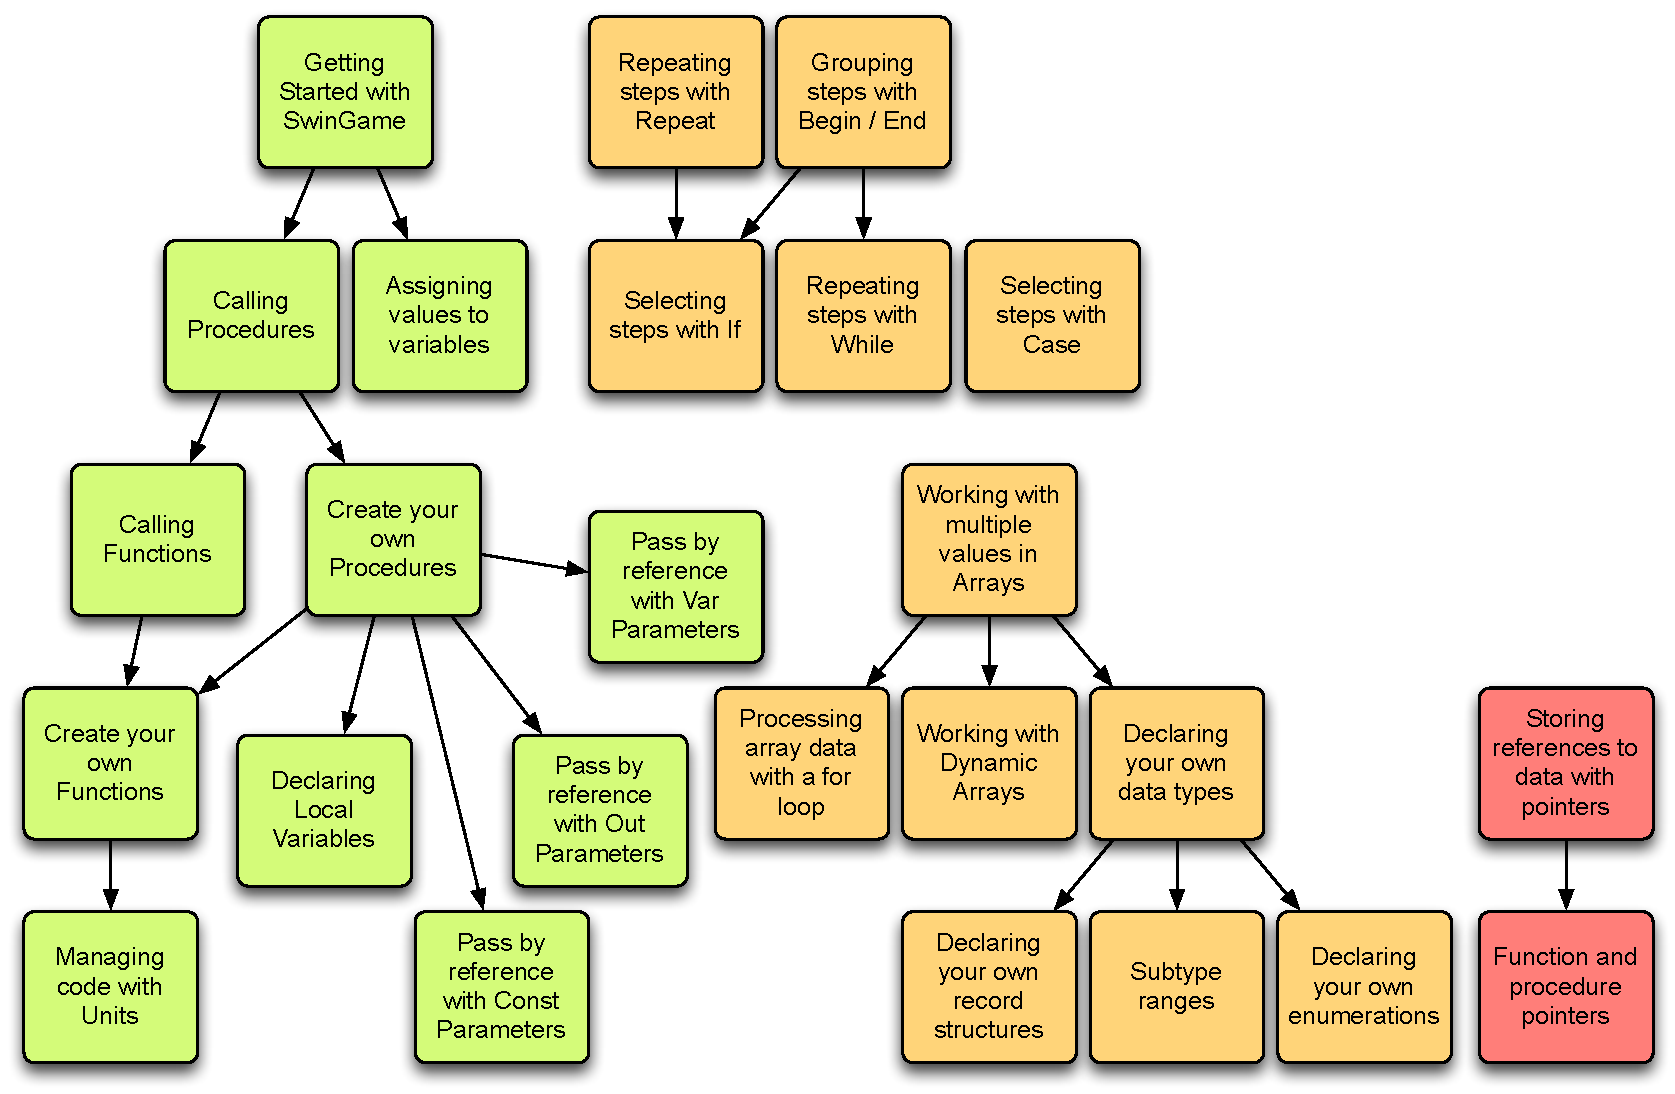
\includegraphics[width=\textwidth]{PodCasts1}
  \caption{Episodes from Learning Programming with SwinGame video podcasts from iTunesU. The different colours represent the three progressively deeper levels, with the expectation viewers would watch all episodes shown in green before progressing to the ones marked in orange, and all of these would be viewed before the podcasts marked in red.}
  \label{fig:podcasts}
\end{figure}

% subsection learning_programming_with_swingame (end)

\subsection{Introductory Programming} % (fold)
\label{sub:introductory_programming}

Introductory Programming was the last series created, and contained seven episodes that were aligned with the first seven chapters of the Programming Arcana. Each video podcast presented concepts using a number of slides, taken from associated lectures, and included programming demonstrations in the C and C++ languages. The goal for this series was to provide students with a summary of the concepts from each lecture. Episodes lasted between seventeen and thirty eight minutes.

% subsection introductory_programming (end)

\subsection{Supporting Multiple Modes of Learning} % (fold)
\label{sub:supporting_multiple_modes_of_learning}

All three podcast series have been used to support students learning in the example units discussed in \cref{cha:example_impl}. The podcasts provided students with an alternative medium for approaching the concepts and syntax that was included in the Programming Arcana, with the expectation that students would be able to use both resources to support the construction of their knowledge.

% subsection supporting_multiple_modes_of_learning (end)

% subsection vodcasts (end)

% section itunesu_vodcasts_to_support_ (end)

\section{A Game Library to Support Procedures First} % (fold)
\label{sec:swingame}

With the procedures first approach to teaching introductory programming, students are introduced to calling and creating procedures before being introduced to other programming concepts. This approach promotes a focus on \textbf{sequence} in these early tasks, with students creating procedures to group together a sequence of procedure calls that perform a certain task. 

The challenge with this approach, as identified by \citet{Pattis:1993}, is finding meaningful tasks for students to perform. SwinGame was created to help address this issue, and to provide students with resources that would enable them to create more engaging programs.

SwinGame is a game development library designed to support the teaching of introductory programming. Commercial game development tools focus on productivity, removing control from the programmer in order to improve productivity and avoid boilerplate code. The goals of SwinGame focus on enabling students to explore programming concepts, while at the same time creating programs that are fun and engaging. 

The goals of SwinGame are to:
\begin{itemize}[noitemsep, nolistsep]
   \item Support beginner programmers.
   \item Provide functions, procedures, and custom types to enable the creation of small two dimensional games.
   \item Give full control of the program to the developer, requiring explicit requests to perform any actions.
   \item Enable simple cross platform game development, with support for a range of operating systems.
   \item Provide support for a range of programming languages.
   \item Be implemented in such a way that it can be extended by students.
\end{itemize} 


\subsection{Supporting Early Exercises and Lecture Demonstrations} % (fold)
\label{sub:supporting_early_exercises}

SwinGame was used to support the early exercises in the teaching and learning activities for the introductory programming unit described in \cref{cha:example_impl}. For example, procedures were introduced in Week 1 where students developed a small program that drew a house, the resulting code from this exercise is shown in \lref{lst:house_drawing}. This task aimed to focus students on concepts related to procedure declarations, procedure calls and instruction sequence. Sequence was explored by adjusting the order of the instructions in the program, and examining the results on the images drawn. The core exercises in Week 1 then built on this, having students complete a program that used images and sound effects to deliver a joke, the starting code for which is shown in \lref{lst:joke}. Screen-shots of the resulting programs are shown in \fref{fig:week1_progs}.

\passection{lst:house_drawing}{The Pascal code for the House Drawing laboratory exercise from the introductory programming unit. In this program students explored concepts related to procedures and sequence.}{\pascode{Figures/Supporting/HouseDrawing.pas}}

\passection{lst:joke}{The core exercise in Week 1 of the introductory programming unit had students complete a program that told a joke. This included code to draw images, play sound effects and draw text.}{\pascode{Figures/Supporting/KnockKnock.pas}}

\begin{figure}[thb]
  \centering
  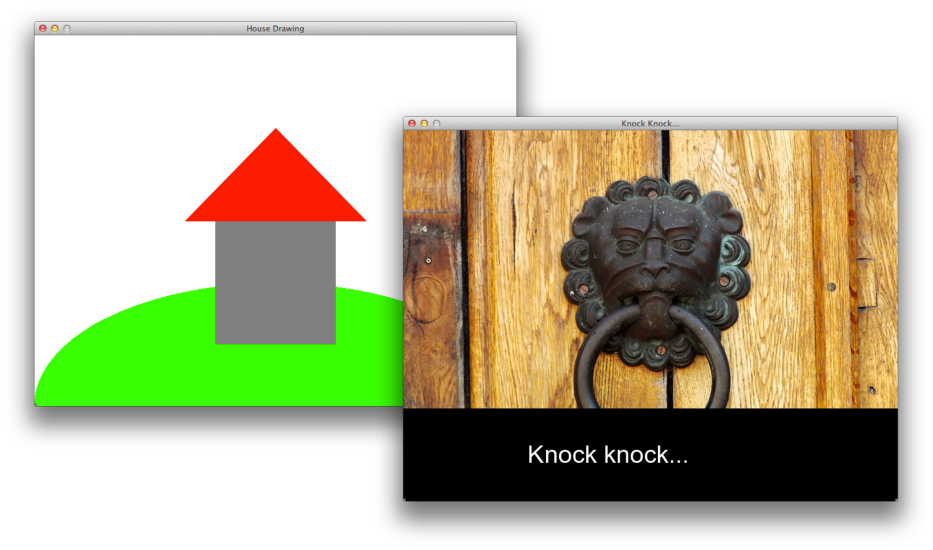
\includegraphics[width=\textwidth]{Week1Progs}
  \caption{The programs created in Week 1 of the introductory programming unit}
  \label{fig:week1_progs}
\end{figure}

With the students in full control of their programs, any form of user interaction required students to implement their own event handling loop. This provided a convenient motivation for control flow mechanisms in Week 3 of introductory programming. By this point, students could create parametrised procedures to draw shapes, but program duration was always set by the length of the delay coded into the sequence. By introducing \textbf{repetition} it became possible to keep a window open \emph{until} the user asked for it to close. With \textbf{selection} user actions could then be responded to, updating values in variables that changed how things were drawn on the screen.

The visual nature of the games developed with SwinGame helped create a more engaging atmosphere in the lectures. By creating visual programs, the lecture demonstration code could be designed and implemented \emph{with} the students. For example, in Week 3 of the introductory programming unit the lecture demonstration created a small program where the user could move a light around the screen and turn it on and off. The code in \lref{lst:lights} shows a part of the code developed in this lecture. The program was created iteratively, involving the students at each stage.

\begin{enumerate}[noitemsep, nolistsep]
  \item Initially the program was developed using concepts from previous week, with the code implementing the \texttt{DrawLight} procedure. At this stage a call to \texttt{Delay} was used to keep the program open for a short period.
  \item The first problem was highlighted by explaining how the program worked, while it was running. Half way through the explanation the program ended, leading to the question ``How can we keep the program open until we want it to close?''. Via various prompts the event loop was described, and coded as the repeat loop in main. Counting out a period longer than the previous delay highlighted that the new code had solved the old problem, and the class discussed what was actually happening behind the scenes to enable this. Closing the window demonstrated the ending of the repeat loop.
  \item The next problem was to make the program more interactive: ``Wouldn't it be good to be able to turn the light on and off?''. This lead to a discussion of what needed to \emph{vary} in the program, and the addition of the \texttt{lightIsOn} variable in \texttt{Main}. This was set to false when the program started, and its state was flipped (on to off, and visa versa) in the repeat loop.
  \item Running the program had an \emph{interesting} effect, as the light flickered between its two states. Questions started with ``Do we always want to change the state of the light?'', and eventually lead to ``So, you only want to change the state of the light \textbf{if} the user has typed the space bar?'' and its follow on ``How can we achieve this in our code?''. After reviewing selection, and the syntax for the if statement, the assignment statement that changed the lights state was put within an if statement. The program was executed and the results discussed.
  \item Other features added in a similar style, each focusing on the application of the concepts to solve a problem or to introduce a new feature.  
\end{enumerate}


\passection{lst:lights}{The final code from the lecture example developed with students in the Week 3 lecture of the introductory programming unit. The program shows a light bulb image that can be turned on and off with the mouse and space bar, and moved around the screen using arrow keys.}{\pascode{Figures/Supporting/Lights.pas}}

Each week's lecture demonstrations followed a similar sequence of events. SwinGame enabled these interactive through its requirement for explicit control, and its support for multimedia resources. In later weeks lecture demonstrations involved the development, and weekly expansion of a small game. These games were proposed by students, with appropriate guidance. Students supplied images and sound effects, suggested features, discussed implementation strategies and were engaged in the iterative implementation of these games. \fref{fig:games} shows screen-shots of two games developed in the lectures, the code of which was then shared with the students.

\begin{figure}[thbp]
  \centering
  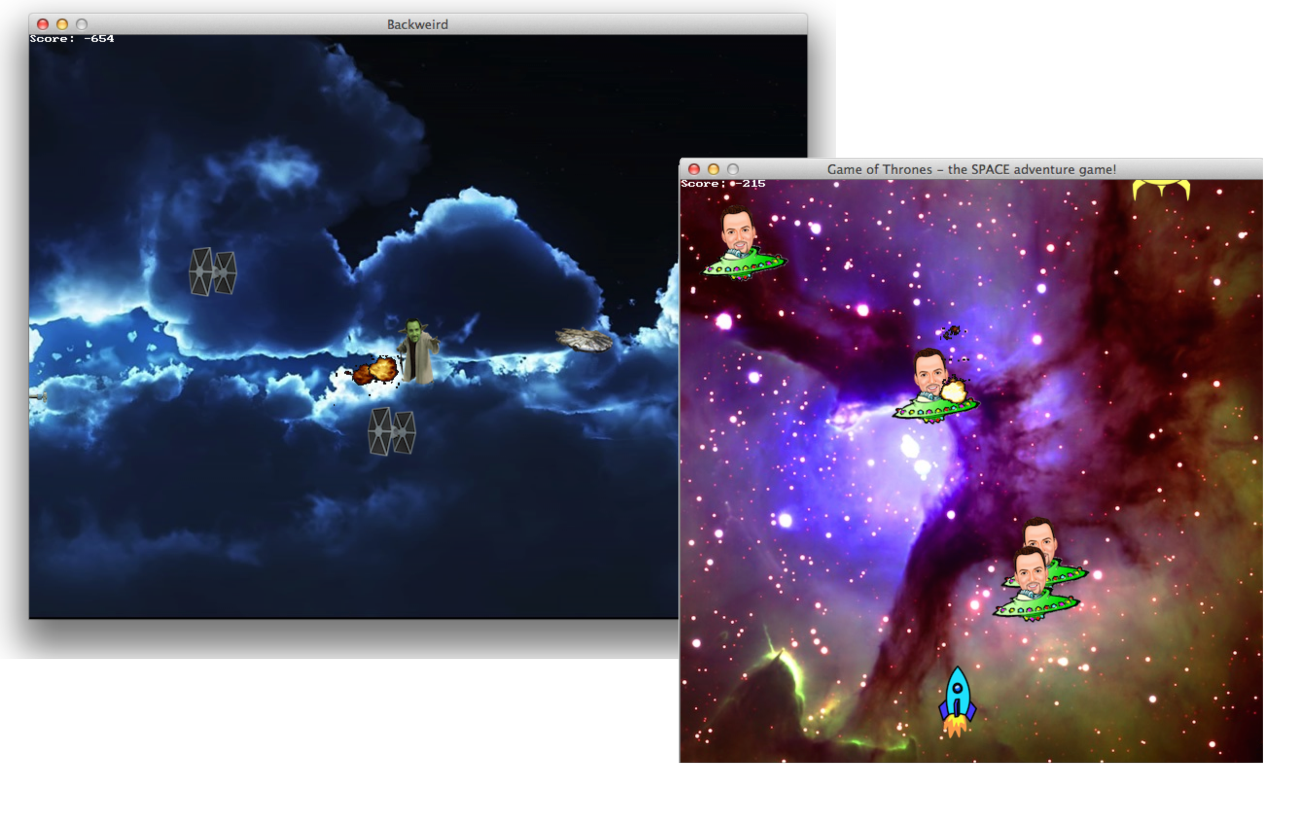
\includegraphics[width=\textwidth]{Games}
  \caption{Games developed with students across a number of weeks in introductory programming}
  \label{fig:games}
\end{figure}

% subsection supporting_early_exercises (end)

\subsection{Supporting Custom Projects} % (fold)
\label{sub:supporting_custom_projects}

As well as supporting the delivery of lecture material, SwinGame provided students with a wide range of capabilities they could use in the creation of their \emph{custom projects}. To be eligible for at least a Distinction grade, students needed to demonstrate they could apply the concepts from the unit to the development of a program of their own design. While there was no requirement for students to use SwinGame, most chose to create a game using SwinGame.

To help support this, the SwinGame functionality was documented on the SwinGame website (\url{http://swingame.com}), as shown in \fref{fig:website}. The website was created to list the SwinGame functions and procedures, and additional documentation was added for some of the more common tasks. The site also provided a means of distributing the SwinGame library to a wider audience.

\begin{figure}[thbp]
  \centering
  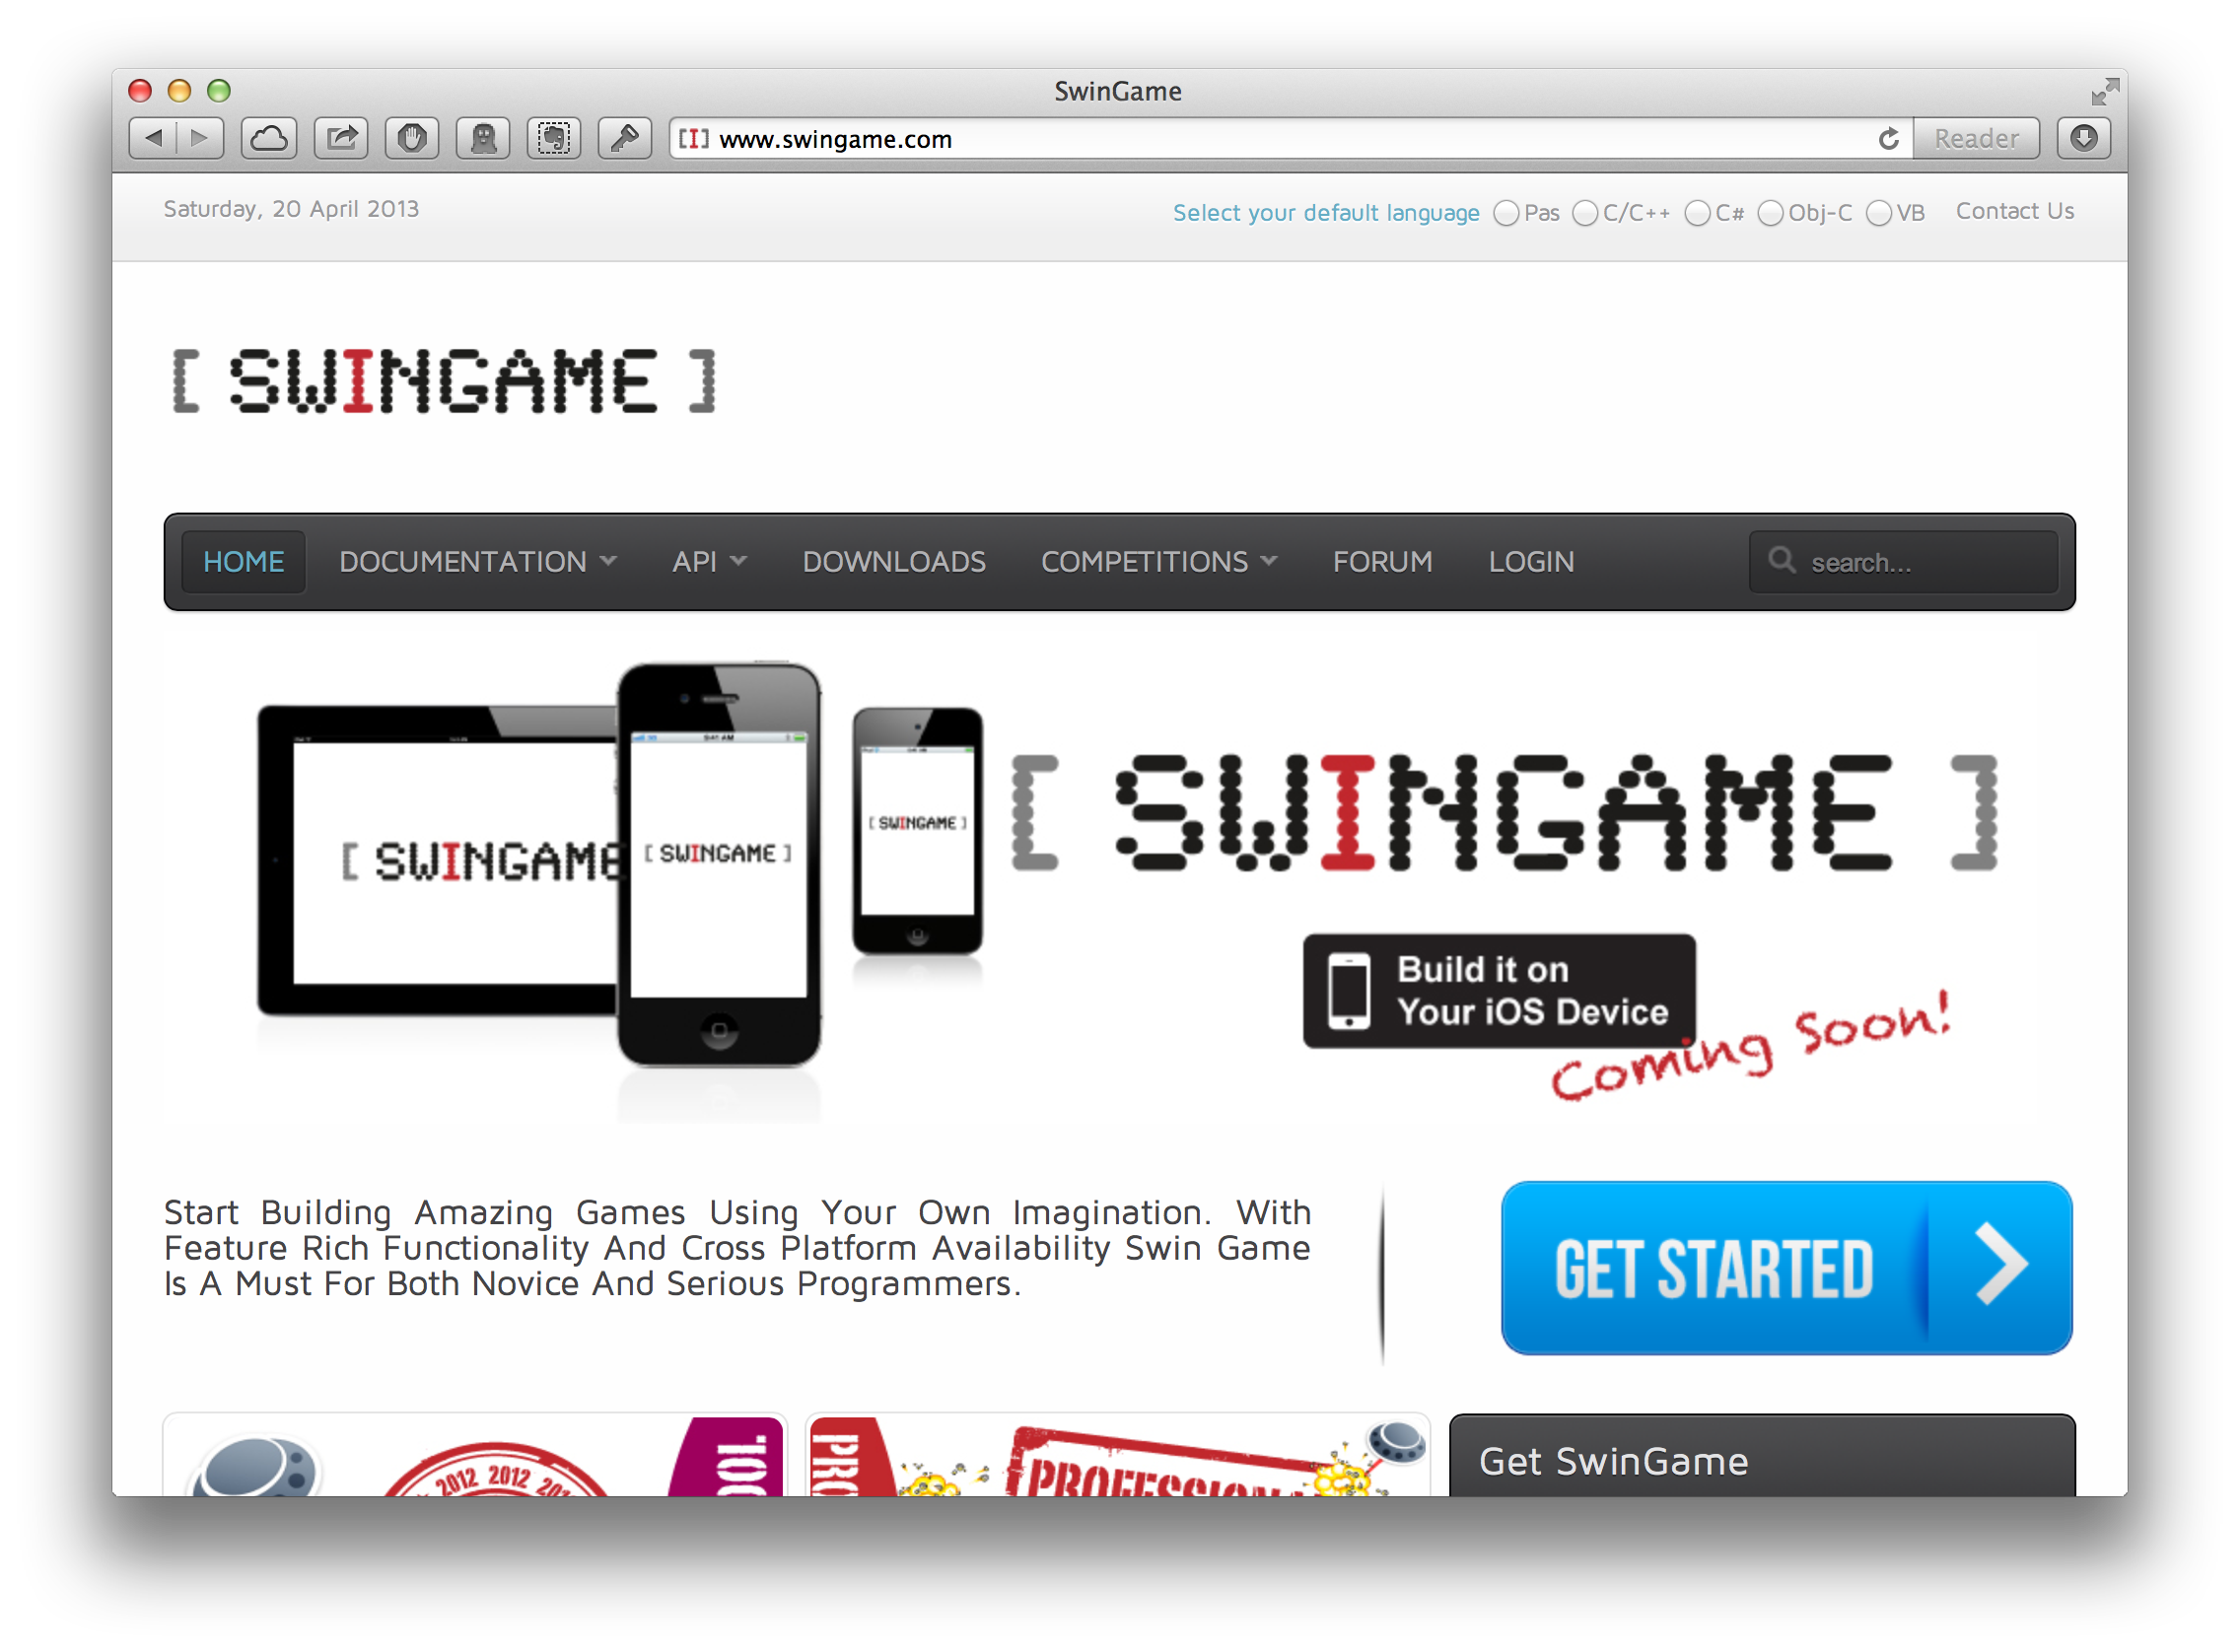
\includegraphics[width=0.9\textwidth]{SwinGame}
  \caption{The SwinGame website provides a means of distributing SwinGame and its documentation}
  \label{fig:website}
\end{figure}

% subsection supporting_custom_projects (end)

\subsection{Developing SwinGame and its Documentation} % (fold)
\label{sub:developing_swingame_and_its_documentation}

SwinGame was developed through the collaboration of both staff and students over a number of years. At the end of each year, students were invited to work on enhancing SwinGame's implementation and documentation. This provided an opportunity for staff to work closely with students, and for students to further develop their software development skills outside of the standard teaching periods.

% subsection developing_swingame_and_its_documentation (end)

\subsection{Supporting Multiple Languages} % (fold)
\label{sub:supporting_multiple_languages}

With the introductory programming unit using two programming languages, and object oriented programming using four, SwinGame was required to be accessible from a range of programming languages. This included both procedural and object oriented programming languages. To achieve this goal a number of tools were created to simplify the process of creating programming language specific version of SwinGame.

SwinGame's core logic is implemented via a number of modules, one for each aspect of the SwinGame functionality. These modules can be accessed via language specific wrappers as shown in \fref{fig:swingame_arch}. Each wrapper mimic the SwinGame logic, and act as adapters that perform any required transformation of data between the program's runtime environment and the native SwinGame library, which is accessed via the SwinGame Library Interface. This interface consolidates all of the SwinGame functionality and exposes it as a native library, it also acts as an adapter that converts SwinGame types to, and from, appropriate native representations that can be exchanged across the native interface. 

\begin{figure}[thbp]
  \centering
  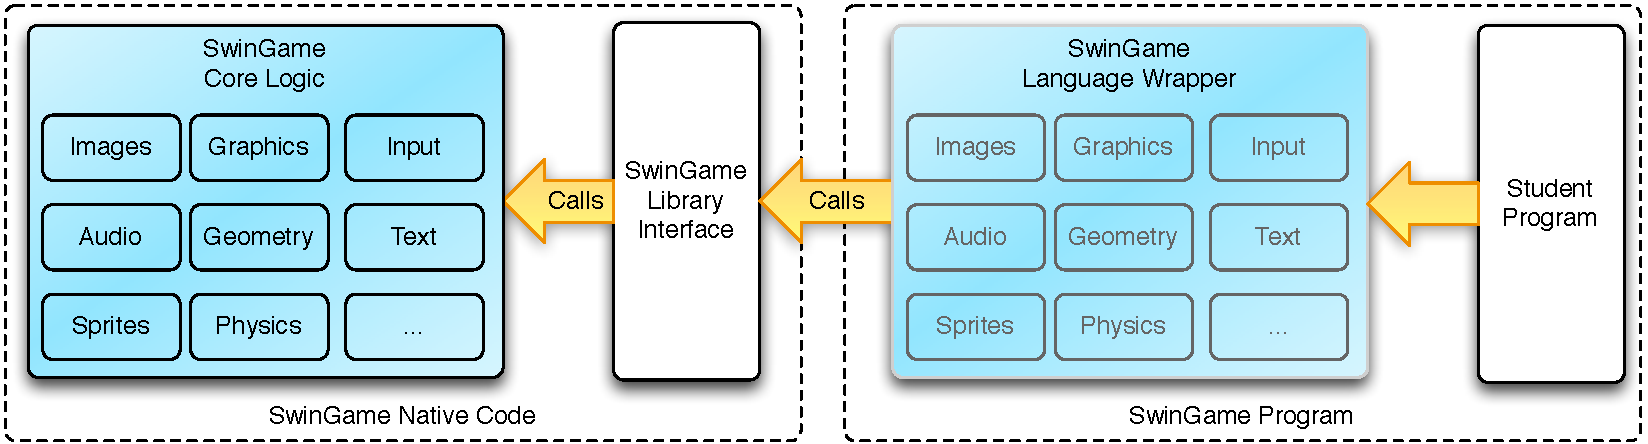
\includegraphics[width=\textwidth]{SwinGameArch}
  \caption{SwinGame core logic is implemented in a number of modules that are accessible via language specific wrappers }
  \label{fig:swingame_arch}
\end{figure}

To ease the creation of the language specific wrappers a translator was created that read the source code for the SwinGame core logic and output the SwinGame Library Interface, a number of matching language specific wrappers, and the programmer documentation for the SwinGame website as shown in \fref{fig:swingame_trans}. This ensured consistency between the wrapper, SwinGame Library Interface and the documentation while allowing the development of SwinGame to focus on enhancing the core logic.

\begin{figure}[thbp]
  \centering
  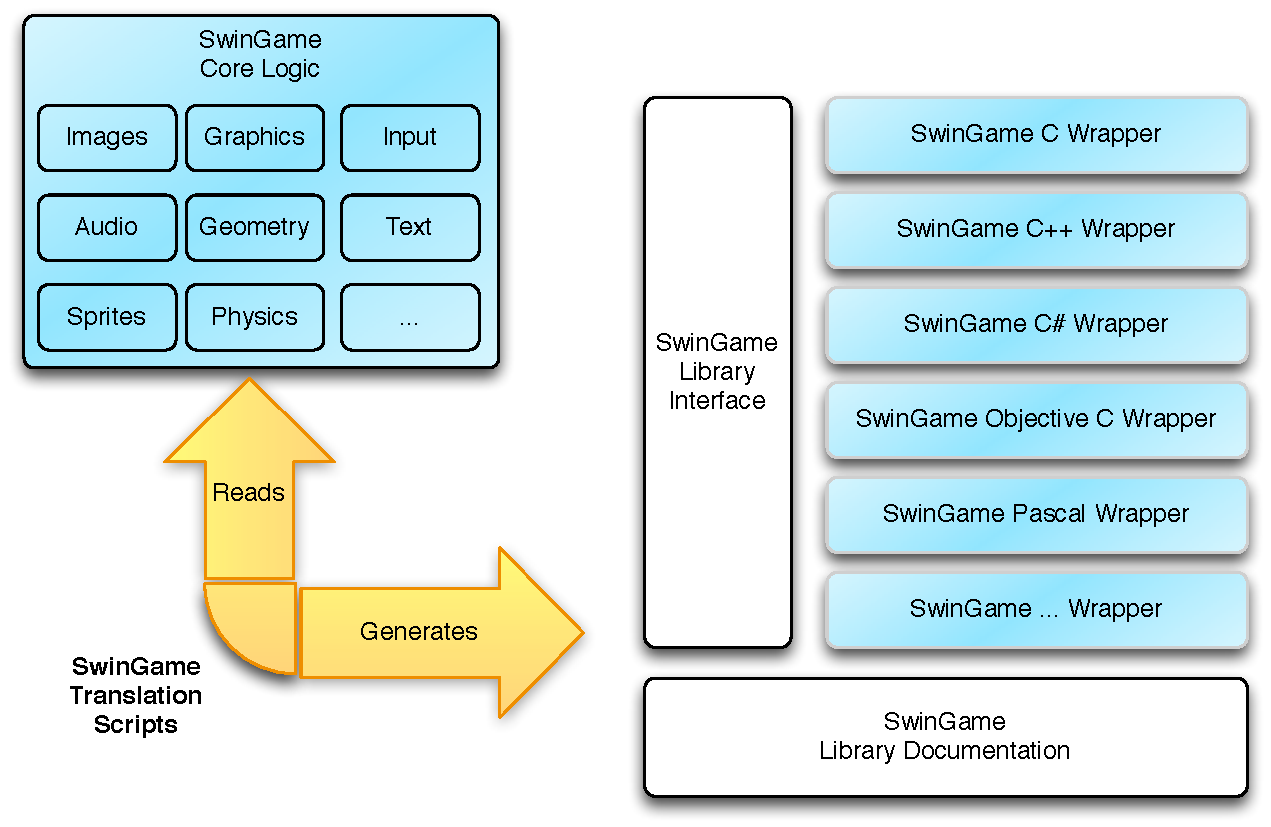
\includegraphics[width=\textwidth]{SwinGameTranslator}
  \caption{SwinGame's language specific wrappers, library interface and programmer documentation are all generated from its source code. The translator reads the source code, and outputs the SwinGame library, and language specific wrappers for a range of programming languages.}
  \label{fig:swingame_trans}
\end{figure}

SwinGame's language translation scripts requires additional information to enable the construction of the various artefacts. It was decided to store this additional information using attributes in comments in the code for the core logic. These special comments started with \texttt{///} and contained documentation as well as other attributes. These attributes were marked using the \texttt{@} symbol followed by a attribute identifier and a number of values. Two example functions from the SwinGame core logic are shown in \fref{lst:audio}, and \tref{tbl:attributes} provides details of the attributes shown.

\passection{lst:audio}{Example of markup language used to annotate SwinGame core logic to enable generation of language specific wrappers.}{\pascode{Figures/Supporting/Audio.pas}}

\begin{table}[hbp]
    \footnotesize
    \centering
    \caption{The main language translation attributes, their format and purpose.}
    \label{tbl:attributes}
    \begin{tabular}{l|l|p{8cm}}
    Attribute & Format & Purpose \\
    \hline
    \texttt{@param} & \texttt{@param name docs} & Provides additional documentation for a parameter. \\
    \texttt{@lib} & \texttt{@lib} & Indicates the function/procedure should appear in the SwinGame Library Interface. \\
    ~ & \texttt{@lib call} & Indicates that the wrapper should call another function/procedure from the SwinGame Library Interface. \\
    \texttt{@uname} & \texttt{@uname name} & Function and procedure names in the SwinGame Library Interface, and some wrappers, need to be unique. This attribute provided a unique name for this function or procedure. \\
    \texttt{@sn} & \texttt{@sn format} & Provides a format string for the creation of the Objective C signature for this function/procedure. This allows parameters to be mixed with the name of the method. \\
    \texttt{@class} & \texttt{@class name} & The name of the class to add the method to. \\
    \texttt{@method} & \texttt{@method} & The name of the method to add to the class. \\
    \texttt{@overload} & \texttt{@overload name uname} & Overloads the method name, uname is used in langauges that do not support overloading. \\
    \texttt{@csn} & \texttt{@csn format} & Similar to @sn, providing the format for the Objective C signature for the method added to the class. \\
    \end{tabular}
\end{table}

The \texttt{@lib} parameter determines if the function or procedure is added to the SwinGame Library Interface. When the function or procedure is not to be added, an alternative call is provided. The generated wrapper code is then adjusted to call the appropriate version. The code in \fref{lst:audio} indicates that \texttt{LoadSoundEffect} should be included directly in the interface, whereas this version of the \texttt{PlaySoundEffect} procedure calls \texttt{PlaySoundEffectA} and passes in default values for some parameters.

All SwinGame resources are accessible via pointers, enabling the language translation scripts to create object oriented abstractions, when this is appropriate for the wrapper's programming language. \fref{fig:swingame_wrapper_output} shows illustrates that main components created by the translator. 

Each function and procedure in the core logic is capable of creating two methods in these object oriented language wrappers. The first method is created as a static\footnote{Static in this context is meant to indicate that the method is associated with the class, rather than instances of the class.} member of a class that mirrors the module from the core logic. 

A second method can then be associated with a resource class. The specific class is indicated by the \texttt{@class} attribute. These classes contain a field to track the resource's pointer, and so the method will have one fewer parameters. When this method is called it calls the appropriate method on the wrapper class and passes in the value from the field along with any other parameter values passed to the method.

\begin{figure}[thbp]
  \centering
  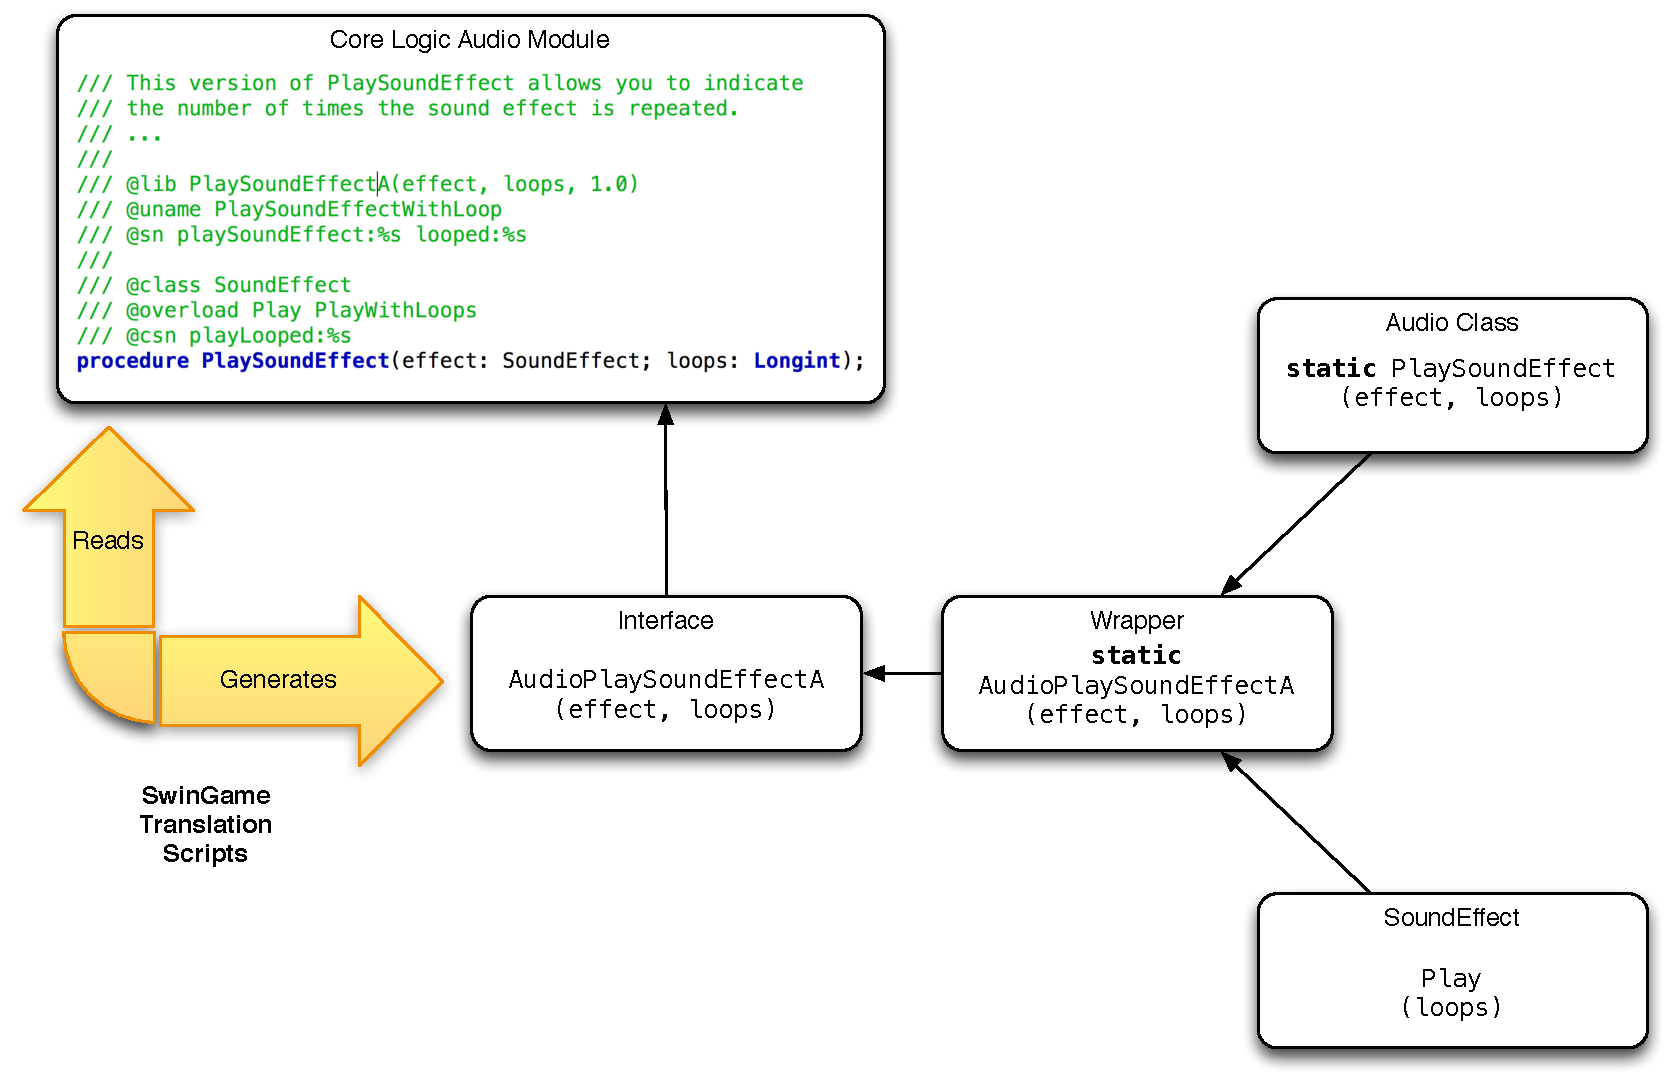
\includegraphics[width=\textwidth]{SwinGameWrapperOutput}
  \caption{Attributes in the core logic code define the generation of a module level wrapper, and the creation of classes for object oriented access to SwinGame resources.}
  \label{fig:swingame_wrapper_output}
\end{figure}

The Objective C syntax required special attention. For example, the procedure PlaySoundEffect shown in \fref{lst:audio} could be called using \texttt{[Audio playSoundEffect:effect looped:3]}. The signature to match this required the parameters to be embedded within the method's name. This was achieved by added \texttt{@sn} and \texttt{@csn} attributes that allow the developer to specify a format string into which the parameter signatures will be injected.

By supporting both procedural and object oriented programming languages, SwinGame was able to be used in both the introductory programming and object oriented programming units. In introductory programming students worked with SwinGame from Week 1, and explored its use from both the Pascal and C programming languages. In the object oriented programming unit, SwinGame provided a familiar framework for students to work with at the start of the teaching period. As the period progressed, students were transitioned away from using SwinGame to encourage them to explore other commercially available libraries by the end of the unit.

% subsection supporting_multiple_languages (end)
\subsection{Supporting What We Teach} % (fold)
\label{sub:supporting_what_we_teach}

SwinGame performed a central role in supporting \emph{what} we taught, as illustrated in \fref{fig:what_we_teach}. SwinGame helped to enable the interactive lectures, and to provided the tools necessary to create engaging examples in the Programming Arcana and the video podcasts. It also provided a consistent library for students as they moved between programming languages.

\begin{figure}[thb]
  \centering
  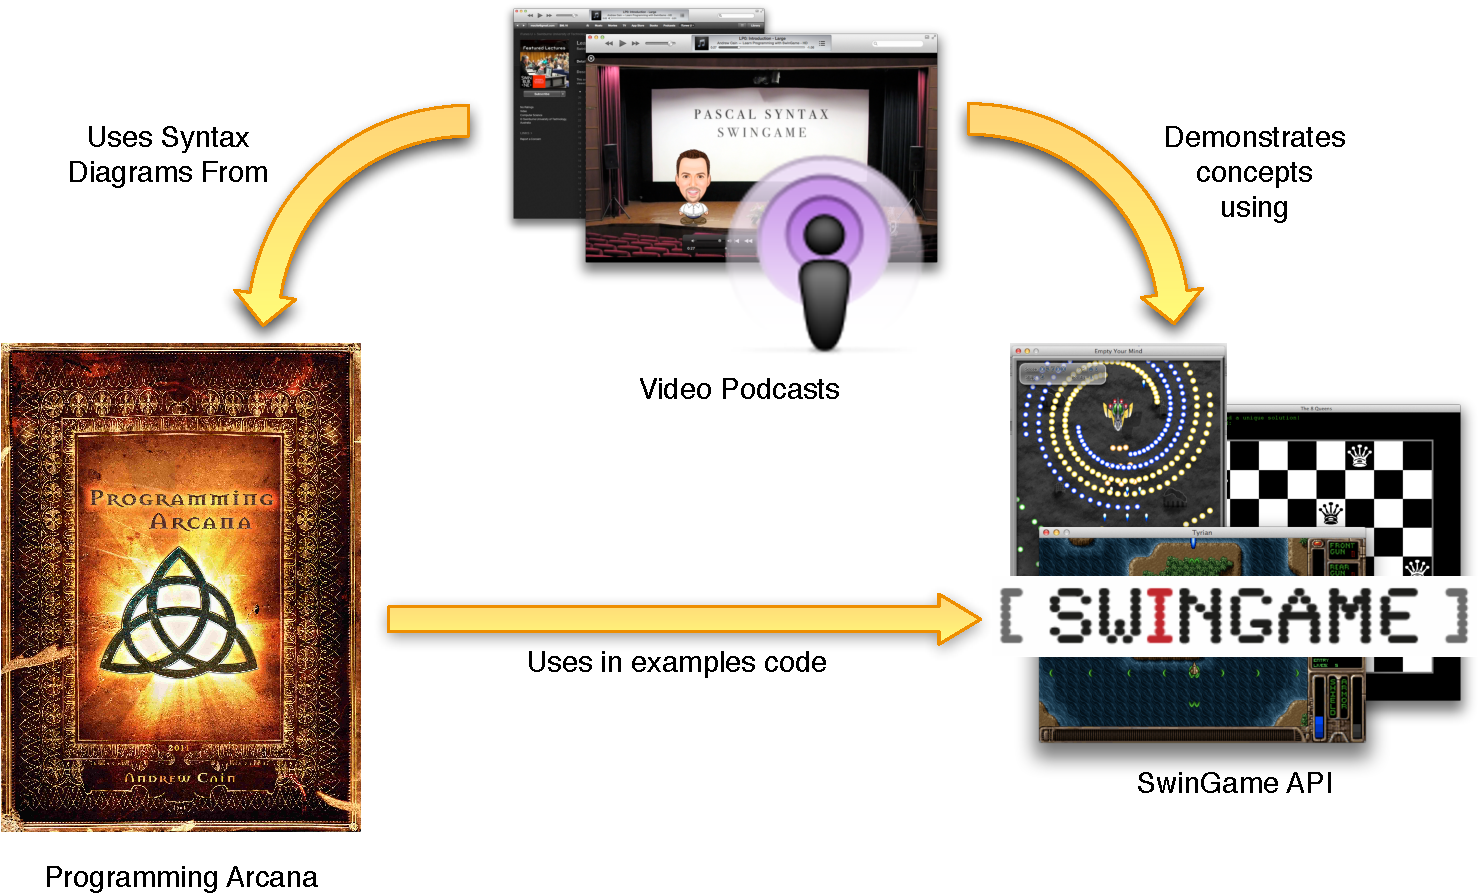
\includegraphics[width=0.8\textwidth]{SupportWhatWeTeach}
  \caption{What we taught was supported by the Programming Arcana, the video podcasts and SwinGame.}
  \label{fig:what_we_teach}
\end{figure}


% subsection supporting_what_we_teach (end)

% section swingame_a_game_library_to_support_procedures_first (end)
\clearpage
\section{Summary} % (fold)
\label{sec:supporting_summary}

This chapter has discussed four resources used to support \emph{how} and \emph{what} we taught in the example units from \cref{cha:example_impl}. \sref{sec:doubtfire} described the Doubtfire tool, used to support the use of formative feedback during the semester. In creating Doubtfire we aimed to provide students with visual feedback on their progress in lieu of marks. The Programming Arcana provided students with details on the concepts, their application, associated syntax, and operation on the notional machine. These same concepts were also supported by video podcasts, providing students with an alternative means of study.

\cref{cha:evaluation} presents an evaluation of these resources, the teaching and learning activities from \cref{cha:example_impl}, and model from \cref{cha:approach}.

% section summary (end)


% chapter supporting_the_curriculum (end)